\chapter{Multiagent Programming with LLMs}\label{ch:seidr}

\todo{Ensure standard nomenclature}

\newcommand{\method}[0]{SEIDR}
\newcommand{\synthesize}[0]{SYNTHESIZE}
\newcommand{\execute}[0]{EXECUTE}
\newcommand{\instruct}[0]{INSTRUCT}
\newcommand{\instructs}[0]{INSTRUCT$^{\text{static}}$}
\newcommand{\instructllm}[0]{INSTRUCT$^{\text{LLM}}$}
\newcommand{\debug}[0]{DEBUG}
\newcommand{\rank}[0]{RANK}
\newcommand{\beamwidth}[0]{W}
\newcommand{\treearity}[0]{N}
\newcommand{\treearitydebug}[0]{N_\text{debug}}
\newcommand{\treearityexplain}[0]{N_\text{explain}}
\newcommand{\treearitydraft}[0]{N_\text{synth}}
\newcommand{\expectedoutput}[0]{O}
\newcommand{\synthmodel}[0]{$p_\text{synth}(\text{code}, \text{descr})$}
\newcommand{\debugmodel}[0]{$p_\text{debug}(\text{code}, \text{descr})$}
\newcommand{\textmodel}[0]{$p_\text{explain}(\text{code}, \text{descr})$}
\newcommand{\synthmodelnoargs}[0]{$p_\text{synth}$}
\newcommand{\debugmodelnoargs}[0]{$p_\text{debug}$}
\newcommand{\textmodelnoargs}[0]{$p_\text{explain}$}

\newcommand{\gpt}[0]{GPT-3.5}
\newcommand{\llama}[0]{Llama~3}
\newcommand{\cpp}[0]{C++}
\newcommand{\py}[0]{Python}
\newcommand{\smalltt}[1]{\texttt{\fontsize{8.5}{9}\selectfont#1}}

\todo{citeself}

\section{Motivation}
There are many ways to start this chapter, but only one honest way: multiple significant advances in large autoregressive language models for code swept the world precisely at the time that work was being completed on chapters \ref{ch:bfpp}-\ref{ch:tree2tree} and were utterly impossible to ignore.

\todo{Rewrite}

\section{Introduction}
\label{sec:seidr-intro}

Automatic programming has been an important goal of the field of artificial intelligence almost since its inception, promising to reduce the workload of software developers by automatically solving some of the tasks they face~\cite{manna1971:automatic}.
More recently, program synthesis has emerged as an interpretable alternative to black-box machine learning methods that lets human experts understand, validate and edit the algorithms generated by artificial intelligence~\cite{bastani2022:interpretable}.
In addition to the scientific benefits of such knowledge, it extends the benefits of machine learning to domains, such as embedded systems where it is technically challenging~\cite{dhar2021:survey} or healthcare where it is avoided for safety reasons~\cite{connolly2023:systematic,jia2022:role}.

The predominant methodology in automatic programming has shifted from deductive programming~\cite{manna1992:fundamentals,alur2015:syntaxguided} to genetic and evolutionary methods~\cite{ahvanooey2019:survey} to, more recently, large autoregressive language models trained on corpora of source code~\cite{xu2022:systematic, zan2023:large} to benefit from their remarkable capability for zero-shot generalization~\cite{chen2021:evaluating}.
However, even state-of-the-art models fine-tuned on a specific class of programming tasks still require a costly filtering step in which the LLM outputs that do not compile or pass tests are discarded~\cite{li2022:competitionlevel}.
These outputs tend to be superficially similar to correct solutions~\cite{ren2020:codebleu,liu2023:your, shirafuji2023:exploring} despite failing to produce the expected output, a phenomenon known as "near-miss syndrome" or "last mile problem"~\cite{bavishi2022:neurosymbolic}. 

Given these challenges, research in machine learning on source code~\cite{allamanis2018:survey} tends to focus on restricted domain-specific languages~\cite{chen2021:latent,polozov2015:flashmeta,liventsev2021:bf} or automating specific parts\footnote{~Similarly to autonomous driving~\cite{grigorescu2020:survey,marcano2020:review}.} of the software development process~\cite{lu2021:codexglue,niu2023:crosscodebench} such as code search~\cite{husain2020:codesearchnet}, code translation~\cite{roziere2020:unsupervised}, detection of issues~\cite{fernandes2016:reviewbased,chakraborty2021:deep}, improvement~\cite{petke2018:genetic} and repair~\cite{legoues2019:automated} rather than fully autonomous programming in a programming language popular with human developers.\footnote{~\url{https://www.tiobe.com/tiobe-index/}}
% ~\cite{:tiobe}.
However, two recent innovations potentially make the latter task tractable.

One is \emph{Synthesize, Execute, Debug}~\cite{gupta2020:synthesize}, a framework that attempts to bridge the "last mile" gap by introducing program repair into the program synthesis algorithm. 
A programming task is specified using both a natural language description and a set of input/output (I/O) pairs that demonstrate what output is expected from the program, thereby combining text-to-code~\cite{iyer2018:mapping} and programming by example~\cite{halbert1984:programming,gulwani2016:programming} paradigms typical for competitive programming~\cite{zavershynskyi2018:naps}.
\emph{Synthesize, Execute, Debug} creates a first draft program using a generative model, compiles and executes it with given input examples.
This is followed by a program repair step to fix the identified errors.

Another relevant innovation is instruction fine-tuned large language models~\cite{ouyang2022:training}. Instruction fine-tuned models use human feedback in their training process and are designed to explicitly or implicitly admit two inputs: a source text (or code) and a textual command instructing the model to edit the source in a particular way, e.g., ``summarize'' or ``translate to Python.''
These models have been shown to be highly successful in automatic program repair~\cite{fan2023:automated}. 
However, given the free-form nature of these instructions,\footnote{~\ag{Throughout this paper we avoid other definitions of \emph{instruction}, such as \emph{an individual operation in code}, to prevent ambiguity.}} how one should engineer instructions that maximize repair performance is an open question. 

These innovations have led to the proposal of a framework, \emph{Synthesize, Execute, Instruct, Debug and Rank}, or \method{}\footnote{~Seiðr also refers to a type of Norse magic~\cite{blain2002:nine} pertaining to predicting and controlling the future, which we deem thematically appropriate.}, initially introduced in our GECCO-2023 paper~\cite{liventsev2023:fully}. 
%The current paper partly reiterates the methodology and findings of~\citep{liventsev2023:fully} and expands on them in this extended version of the original paper.
SEIDR is a multi-agent iterative framework that uses feedback from code execution and failing test cases to update the initially generated buggy code. 
Our initial explorations cover SEIDR with GPT-3 as the bug summarization model and Codex (or GPT-3 trained on code) as program generation and debugging model.  
We test a number of prompting strategies for LLMs to fix a working prompt.
In addition, by modifying the tree-arity parameter (see Section~\ref{sec:seidr-beam-search}), we investigate the trade-off between generating and repairing only one program versus regenerating any program that does not pass all the tests, as well as intermediate configurations, where we build a tree of programs and update the best ones.

While Codex is an early code generation model, the emergence of new models that score better in programming and natural languages motivates further research into the use of \method{} with newer models. 
To study the generalizability of the SEIDR results, we use two other LLMs, Llama 3\footnote{~\url{https://ai.meta.com/blog/meta-llama-3/}} and GPT-3.5,\footnote{~\url{https://openai.com/form/researcher-access-program/}} and an additional dataset, HumanEval-X with different tree-arity parameters~\cite{brown2020:language, chen2021:evaluating, zheng2023:codegeex}. 
Moreover, we build up on the initial experiments with Codex and zoom in on the area with the best-performing tree arities in a hyperparameter search for a better repair-replace trade-off resolution. 

To reflect on the parent selection strategies used in the Rank agent of \method{}, we also explore whether the programs should be chosen based on the average performance across all tests or whether \method{} can benefit from keeping such programs in the loop that fully cover individual tests, but do not perform well on average.
Therefore, as an alternative to the tournament selection, we test the best tree-arity setups with lexicase selection-based ranking.
Moreover, since language models bring in stochasticity, we run the experiments several times to measure the variability of results obtained with fixed hyperparameters and reflect on the stability of experiments.

Overall, the current paper contributes to the field of Large Language Models for Software Engineering (LLM4SE) with a framework for code generation and its iterative repair. 
Compared to the earlier GECCO-2023 paper, this article refines and extends the preliminary results by providing a more in-depth explanation of SEIDR as a multi-agent framework for autonomous programming, extending the original experiments and analysis to include HumanEval-X as an additional benchmark, evaluating GPT-3.5 and Llama 3 as additional LLMs, investigating lexicase selection as an alternative to tournament selection, and conducting a repeatability analysis of the framework’s performance over multiple independent runs. Overall, this extension adds three research questions and doubles the number of configurations considered in these questions compared to our preliminary work. 

Section~\ref{sec:seidr-methodology} presents a framework that adapts \emph{Synthesize, Execute, Debug} to instruction fine-tuned Large Language Models in agents for solving programming tasks in an autonomous fashion. 
We discuss related work in Section~\ref{sec:seidr-related-work}, introduce experiments to explore effective search and prompting strategies for this framework in Section~\ref{sec:seidr-eval}. 
Finally, in Section~\ref{sec:seidr-results} we demonstrate that our framework outperforms conventional automatic programming techniques, such as genetic programming and naive application of large language models that generate one solution per problem without updating it iteratively. 

\section{Methodology}
\label{sec:seidr-methodology}
The proposed five-agent \method{} framework  is summarized in Figure~\ref{fig:method}, which we discuss in detail in Section~\ref{sec:seidr-ingredients}.
In essence, to solve a programming task defined as a text description and a collection of I/O examples, we split I/O examples into prompt and validation sets and use the prompt set in a large language model to \synthesize{} a population of candidate solutions.
We \execute{} the solutions, test them against the validation set, generate a text description of the identified problems used to \instruct{} a large language model to produce repaired candidate solutions similar to the way a human developer \debug{}s a program.
We \rank{} the candidates
by correctness, measured as matching I/O pairs, discard the worst candidates, and repeat until a fully correct solution is found.

\begin{figure*}[t]
    \centering
    % 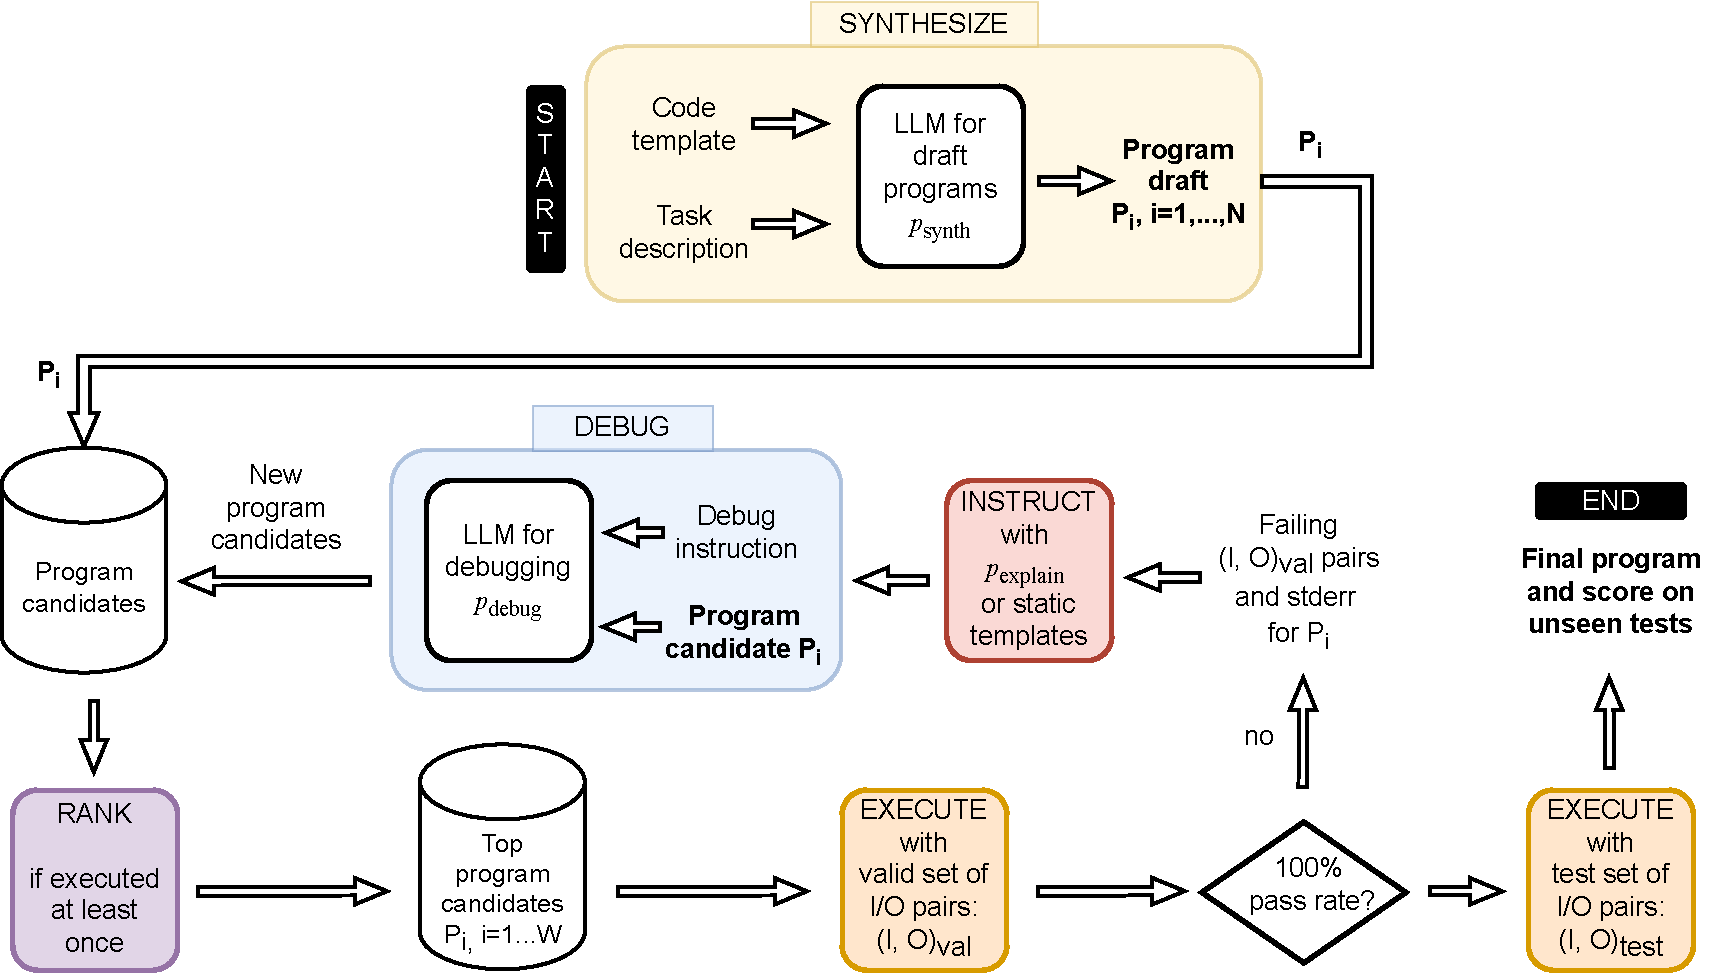
\includegraphics[width=\linewidth,trim={0mm 0mm 0mm 0mm}]{img/methodology/codex-for-psb-seidr-methodology-4.drawio.pdf}
    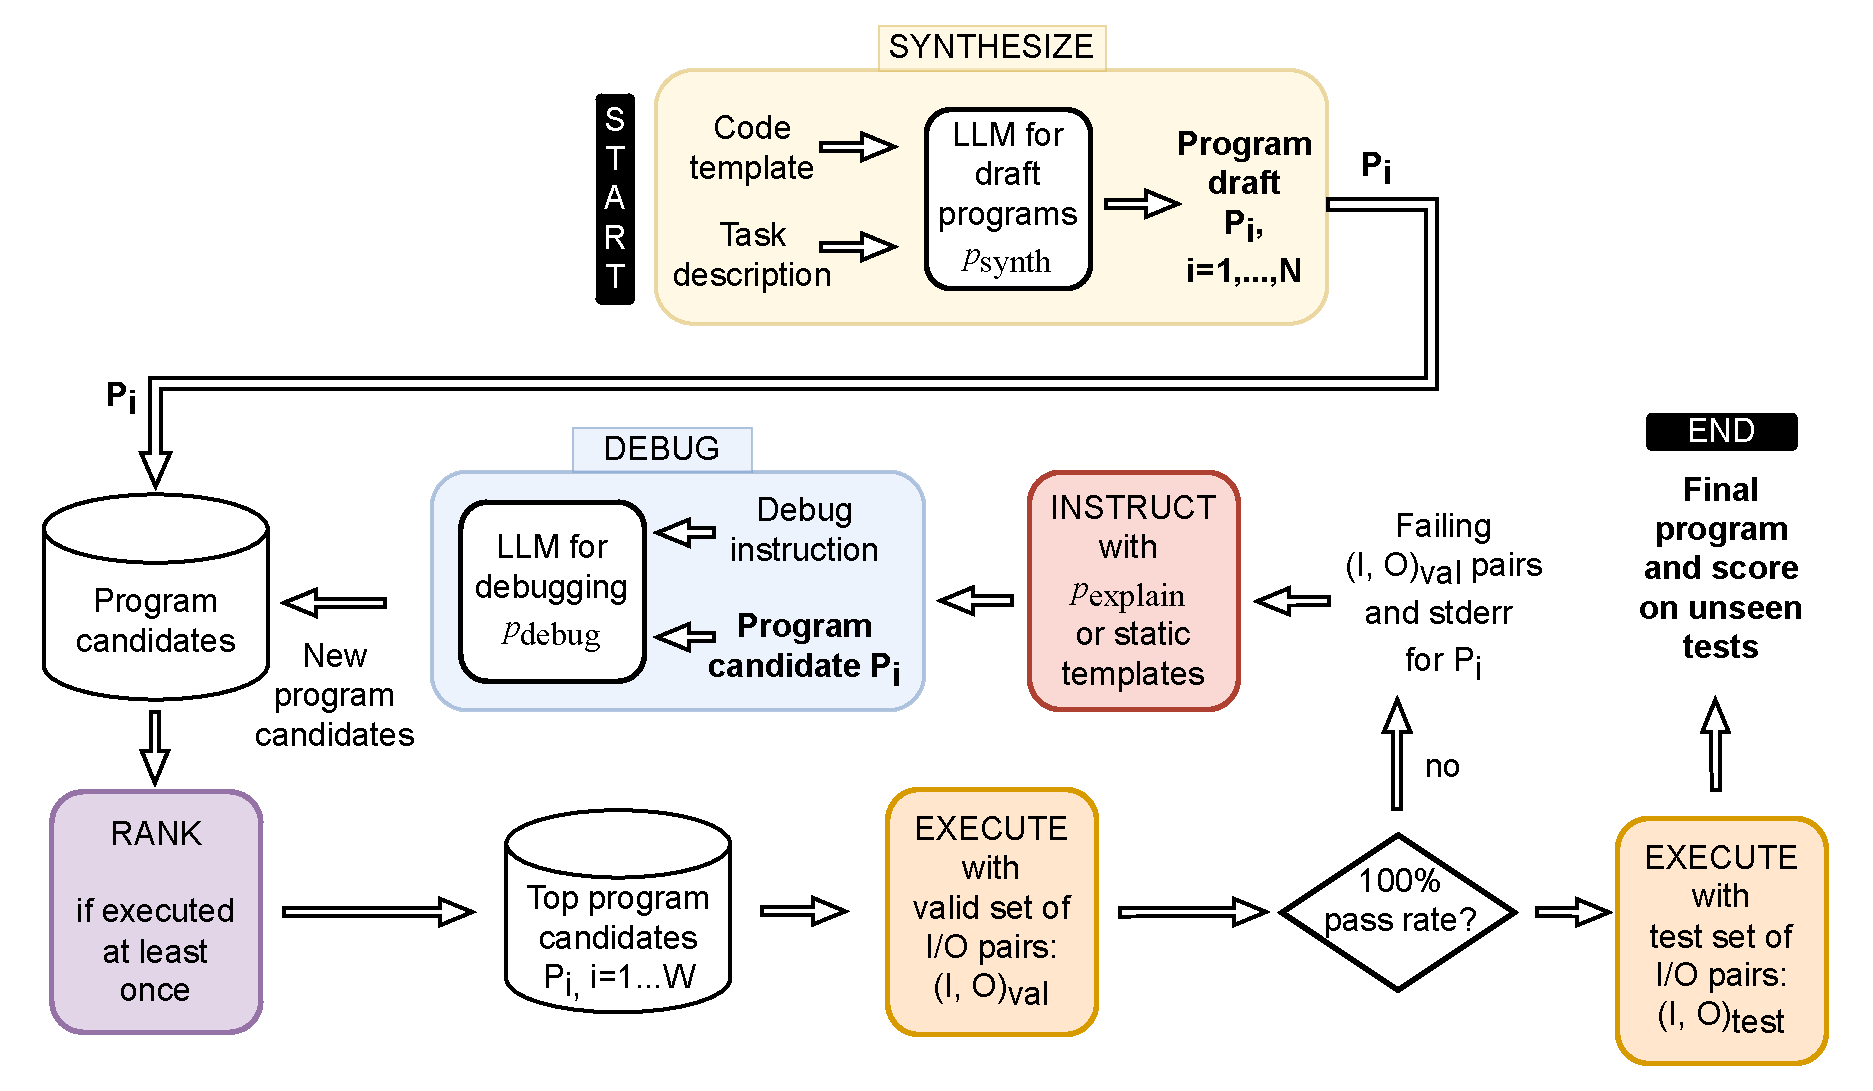
\includegraphics[width=\linewidth,trim={0mm 0mm 0mm 0mm}]{img/methodology/codex-for-psb-seidr-methodology-5.drawio.pdf}
    \caption{Overview of \method{}, a multi-agent iterative framework that uses LLMs to implement the Synthesize, Execute, Instruct, Debug, and Rank feedback loop.}
    \label{fig:method}
\end{figure*}
 

\subsection{Ingredients}
\label{sec:seidr-ingredients}

\method{} makes use of instruction fine-tuned large language models: a \emph{synthesis} model $p_{\text{synth}}(\text{code, }$ descr), a \emph{debugging} model \debugmodel{}, as well as a model \textmodel{} that can be used for writing textual instructions, which are forwarded to the code generation model \debugmodelnoargs{} for code updates. 
Therefore, the design can be described as two agents communicating with each other, whereby one generates code and another provides critical or supervising comments on what should be changed in the generated code. 

The models \synthmodelnoargs{}, \debugmodelnoargs{}, and \textmodelnoargs{} can be either separate models or the same model.
The prerequisites are that \synthmodelnoargs{} and \debugmodelnoargs{} models are able to understand natural language (descr) and partial or full programs (code) and generate code based on them. 
The model \textmodelnoargs{}{} should be able to understand code and natural language and either autocomplete or generate the debugging instruction from scratch. 
Note that \textmodelnoargs{} is optional, since alternatively the debugging instructions can be generated from failing tests using static templates.
%as described in~\cite{liventsev2023:fully}. 
In general, \method{} requires sequence-to-sequence generative models for these agents. 
%In our experiments, we have chosen models \synthmodelnoargs{}, \debugmodelnoargs{}, and \textmodelnoargs{} that are based on the state-of-the-art transformer architecture~\cite{vaswani2017:attention} as a backbone and its subsequent improvements (see Section~\ref{sec:seidr-models}). 
In our experiments, we select models for \synthmodelnoargs{}, \debugmodelnoargs{}, and \textmodelnoargs{} that are based on the state-of-the-art transformer architecture~\cite{vaswani2017:attention} 
%and its subsequent improvements 
(see Section~\ref{sec:seidr-models}). 

Each LLM is a highly parameterised probability distribution over the space of (code, description)-tuples with parameters estimated on a large diverse (i.e., non-task-specific) corpus.
This stochastic nature of language models is an important prerequisite for \method{}, since it allows us to sample batches of diverse candidate solutions from \synthmodelnoargs{}, \debugmodelnoargs{}, and \textmodelnoargs{}. 
We denote the number of outputs generated with $\treearitydraft{},$ $\treearitydebug{},$ and $\treearityexplain{},$ correspondingly.
Moreover, each model generates the most probable and less probable outputs in each batch, which helps diversify problem solving attempts. 
In the following implementation-related subsections, we explain how we vary with the number of candidate solutions, debug instructions, and repairs generated in a batch by each LLM in \method{}.

While \method{} is described here as a multi-agent system, it can equally be seen as a form of evolutionary algorithm or genetic programming, where the initialization and mutation steps of the system are performed by LLMs, \synthmodelnoargs{} and \debugmodelnoargs{}, correspondingly.
Throughout this work, we use agent-oriented programming terminology~\cite{shoham1993:agentoriented} and evolutionary optimization terminology interchangeably to try to bridge the gaps between these domains.

\subsubsection{Synthesize}
\label{sec:seidr-synth}

The framework starts with the \synthesize{} agent, which is responsible for generating initial draft solutions to programming tasks to be repaired in later stages of \method{}.
We start with a basic template for a chosen programming language that contains a number of standard library imports, as shown in Figure~\ref{fig:template}.

\begin{figure}[t]
    \centering
    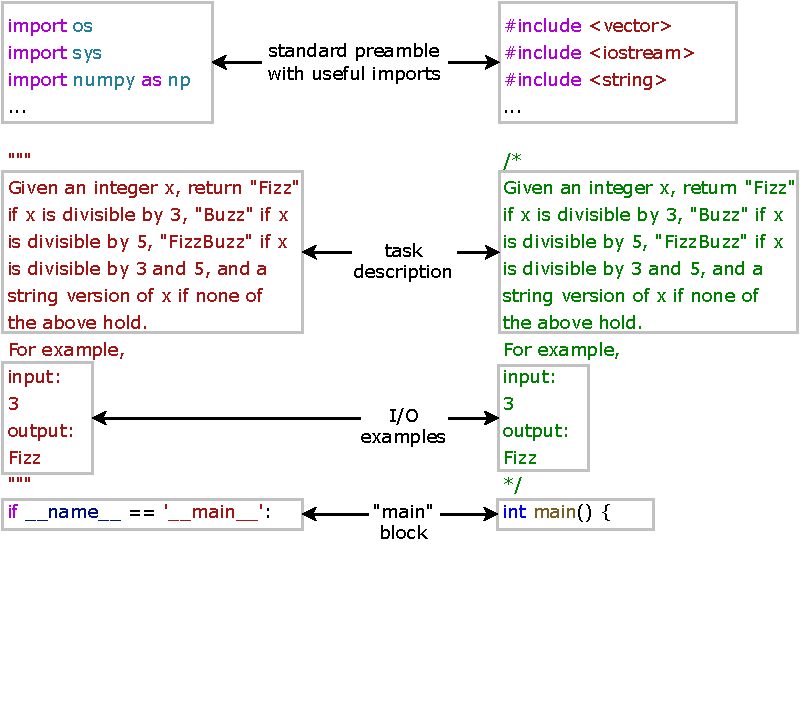
\includegraphics[width=0.8\linewidth, trim={0mm 40mm 0mm 0mm}, clip]{img/templates/Templates-new-v2.pdf}
    \caption{Anatomy of \synthesize{} templates}
    \label{fig:template}
\end{figure}

We populate this template with a comment indicating a text description of a task at hand and several I/O examples from the prompt training set.
We design the templates with prompt engineering guidelines,\footnote{~\url{https://platform.openai.com/docs/guides/prompt-engineering/six-strategies-for-getting-better-results}} and prior work~\cite{debruin2021:autoencoders} in mind.
We then sample $\treearitydraft{}$ programs from \synthmodelnoargs{}, setting \texttt{code} to the populated template and \texttt{description} to the natural language description of what the model should generate.
We use spring sampling:\footnote{~\url{https://vadim.me/publications/spring/}} a temperature-based sampling with a monotonically increasing temperature schedule where the $i$-th program is sampled with temperature $t_i \approx \frac{i-1}{\treearitydraft{}}$ (we use approximate equality to enable efficient implementation by means of batching).
Thus, the sampling procedure for the first programs approximates a deterministic maximum-likelihood estimation.
%Ultimately, this approach ensures that samples are diverse, but always contain the likeliest programs.
In combination with the naturalness principle of source code \cite{allamanis2018:survey,jiang2022:bugs}, this approach ensures that the samples are diverse, but always contain the most likely programs for the given task.

\subsubsection{Execute}
\label{sec:seidr-execute}

The \execute{} agent compiles the programs (if necessary) and launches them using the standard tools for the programming language.
The program is run once for every I/O pair in the validation set. 
Its \texttt{stdin} stream receives all input lines in a given input pair, and its \texttt{stdout} and \texttt{stderr} streams are captured and saved.
We then measure the \emph{score} of the program defined as the accuracy over the output lines, with \expectedoutput{} being the expected output, and $n=\max\{|\expectedoutput{}|, |\text{stdout}|\}$:
\[    
\text{score}(\expectedoutput{}, \text{stdout}) = \frac{\sum^{n}_i{\mathbb{I}[\text{stdout}_i = O_i]}}{n} 
\]
unless \texttt{stderr} is non-empty during compilation or execution, which is considered to indicate failure and is assigned a score of 0.

\subsubsection{Instruct}
\label{sec:seidr-instruct}

The goal of the \instruct{} agent is to provide instructions that summarize bugs in a program candidate and suggest a solution for \debugmodelnoargs{}. 
The resulting instruction(s) with the bug summary should indicate what requirement is violated and instruct the LLM to edit the candidate program accordingly. 
The input to \instruct{} consists of failing I/O pairs from the validation set and \texttt{stderr} output of the candidate execution. 
In order to represent this heterogeneous input as text that can be further processed by an LLM, we use template engines that replace placeholders in files or strings with input values and return a formatted string. 
In recent chat- and instruction-based LLMs, the terms \emph{template engine} and \emph{prompt template} are used interchangeably.

We consider two different designs of the \instruct{} agent: \instructs{} and \instructllm{} shown in Figure~\ref{fig:method-instruct}. 
In both cases, if \texttt{stderr} is not empty, i.e., execution exits with code 0 before getting any output to compare it with the expected output, the \texttt{stderr}-based Template engine generates the instruction to fix the error. 
However, the designs differ in the way they transform failing I/O pairs to generate instructions in case \texttt{stderr} is empty.

\begin{figure*}[t]
    \centering
    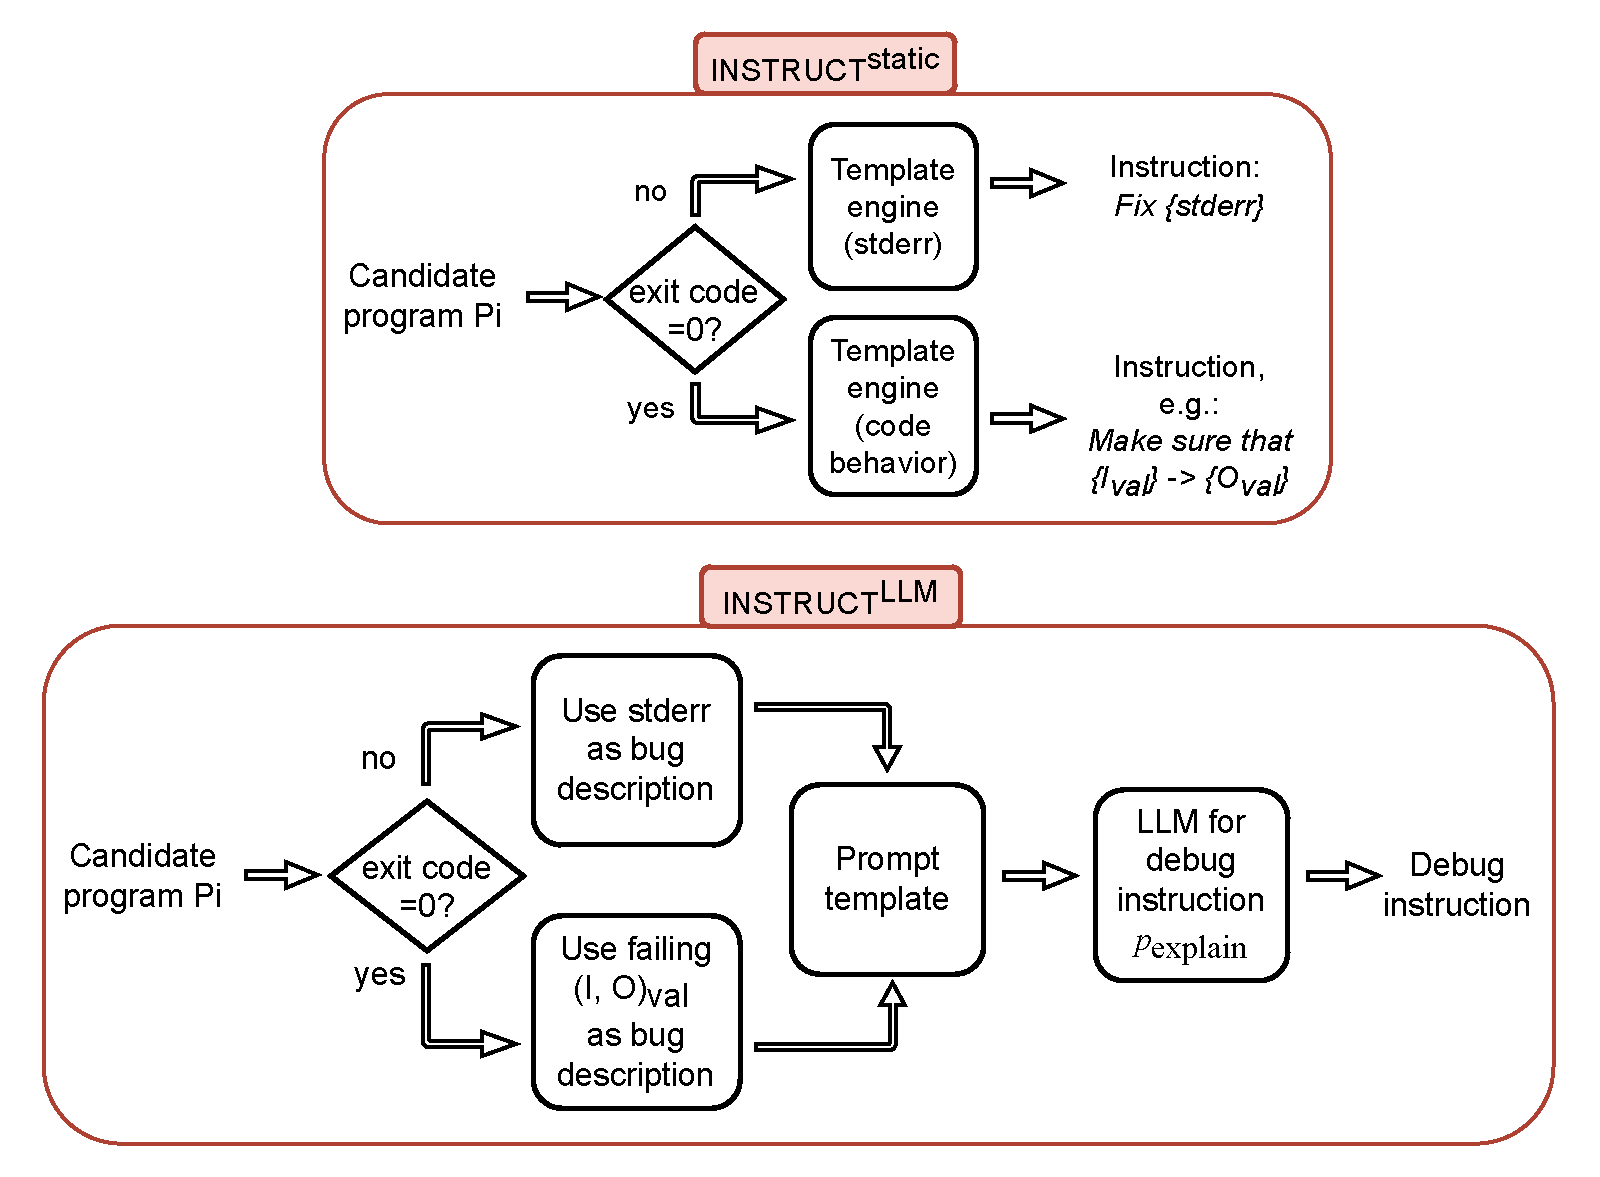
\includegraphics[width=0.85\linewidth,trim={0mm 0mm 0mm 0mm}]{img/methodology/codex-for-psb-seidr-instruct-2.drawio.pdf}
    \caption{Overview of the two designs for the \instruct{} agent.}
    \label{fig:method-instruct}
    % \vspace*{-3ex}
\end{figure*}

\instructs{} uses a fixed template and substitutes placeholders for input and output with the corresponding strings of the first failing test case in its template engine.
For example, we show the resulting instruction for an exemplar template in Figure~\ref{fig:method-instruct}.
In contrast, \instructllm{} uses the failing I/O pair in the LLM for text completion, thereby prompting the text LLM to produce the bug explanation and a summary for debugging. 
In addition to providing a failing test case or \texttt{stderr}, one may choose to give the model \textmodelnoargs{} more context, such as the problem name, task description and the code generated so far. 
Each call to \textmodelnoargs{} can result in $\treearityexplain{}\ge1$ instructions, a batch output of an LLM.
The prompt templates used for the experiments are detailed in Section~\ref{sec:seidr-prompts}.

% An exemplar output of the code behavior template engine in Figure~\ref{fig:method-instruct} describes that the code returns output O instead of expected output O$_{\text{val}}$ for the failing test case with input string I$_{\text{val}}.$
% The LLM is then prompted to auto-complete this description of program behavior with the bug summary. 
% The bug summary is passed further to the next template engine that uses it as debugging instruction, such as ``\emph{Fix \{bug summary\}}''.







\subsubsection{Debug}

The main component of \method{} which addresses the ``near-miss syndrome'' is the \debug{} agent.  
This agent iterates over all programs in the population to repair candidate programs and pass more tests. 
It uses the instructions written by \instruct{} to sample from the \debugmodelnoargs{} model $\treearitydebug{}$ times
to repair each candidate and create a new population of \treearity{} candidates.
For \debugmodelnoargs{}, the parameter \texttt{code} is set to the current version of the candidate solution and \texttt{descr} to the output of \instruct{} and any additional context chosen for a specific implementation.
The current generation of candidates is then replaced by \treearity{} outputs of \debug{}.

\subsubsection{Rank}

The \rank{} agent implements what is known in genetic programming as \emph{parent selection}~\cite{koza1994:genetic}: it selects the best $\beamwidth{}$ programs to be further improved by the \debug{} agent.
We consider two different parent selection algorithms: tournament selection and lexicase selection. 
See Section~\ref{sec:seidr-lexicase-results} for their empirical comparison.

\emph{Tournament selection} variant used in this work sorts the programs according to their average test score and selects top $\beamwidth{}$ candidates. 
% Such ranking approach is a \emph{quality-based} selection method.
The programs are selected based on the intuition that repair of the best so far (but imperfect) programs begets good programs. 
The simple ranking is also referred to as \emph{tournament selection}, where the best-performing candidates are chosen to participate in the next round.  
In the classical tournament selection, the first step is to draw $n$ random candidates from the population. 
In our implementation, the first step is to generate exactly $n$ candidates that are needed for the next round. 
This approach prioritizes candidates that perform the best on average over all tests.
At the same time, tournament selection does not favor candidates that pass fully one or several tests but may not have a high average test pass rate score. 

\emph{Lexicase selection}~\cite{helmuth2015:solving} is a ranking approach that maximizes the diversity of selected candidates in addition to their metric-based score.
Lexicase selection ensures diversity by keeping the program candidates that perform the best on unique tests as opposed to the program candidates that perform best on average over all tests.
The algorithm is as follows:
\begin{enumerate}

\setlength{\parskip}{0pt}
\setlength\itemsep{0pt}

    \item randomly shuffle the set of tests;
    \item select a program with the best score on test 1;
    \item if several programs are tied, resolve the tie by selecting the best program on test 2;
    \item repeat for tests $3,4,\dots,$ until only one program is left;
    \item mark this program as "selected";
    \item if less than $\beamwidth$ programs are selected, go back to step 1.
\end{enumerate}
This ensures that even if the average quality of selected candidates is lower, the batch of $\beamwidth{}$ programs collectively contains a higher number of requisite "skills", as measured by tests.



\subsection{Meaning of Hyperparameters}
\label{sec:seidr-beam-search}

\begin{figure}[t]
    \centering
    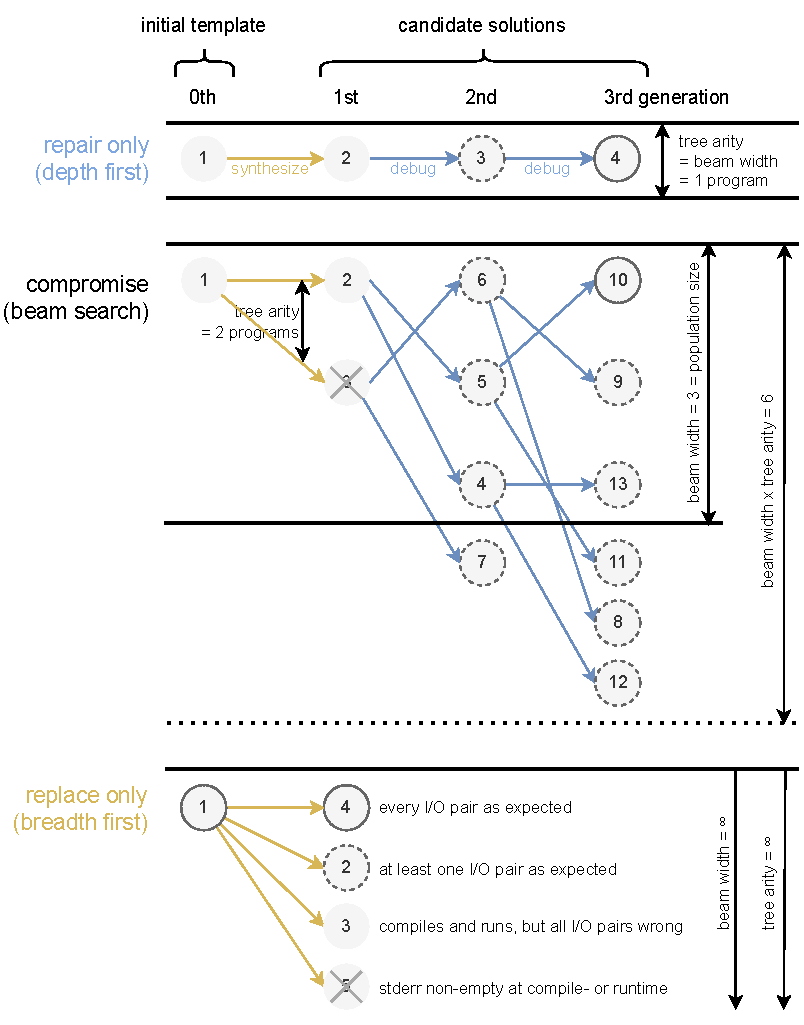
\includegraphics[width=0.7\linewidth, trim={0mm 4mm 0mm 0mm}]{img/beamsearch.pdf}
    \caption{Repair-replace trade-off as a tree search problem.}
    \label{fig:beam-search}
    % \vspace*{-4ex}
\end{figure}

After evaluating a given candidate solution in \execute{}, \method{} supports two approaches to addressing the candidate's flaws:
\begin{itemize}
\setlength{\parskip}{0pt}
\setlength\itemsep{0pt}
  \item \emph{Replace} the candidate with another sample from the current population.
  \item Use \instruct{} and \debug{} to repair the candidate.
\end{itemize}
We refer to this problem as the \emph{repair-replace trade-off}, by analogy with production economics~\cite{jack2000:optimal}. 

How does the choice of hyperparameters $\treearity{},$ the total number of candidate programs in each generation, and $\beamwidth{},$ the number of selected repairs to be preserved in a generation, influence the flow of \method{}?
$\treearity$ and $\beamwidth{}$ act as upper bounds on the \emph{replace} option by limiting the size of the population.
In the edge cases, $\treearity{} = \beamwidth{} = 1$ corresponds to a repair-only process, while $\treearity{} = \beamwidth{} = \infty$ corresponds to replace-only, as illustrated in Figure~\ref{fig:beam-search}. 
Here, the repair-only scenario can also be seen as an LLM-guided random walk~\cite{xia2020:random} and replace-only as random sampling from the LLM.
Strategies with tree arities between $1$ and $\infty$ are  similar to population-based evolutionary algorithms.
Note that $\treearity{}$ is defined by $\treearitydraft{}$ for the initial draft solutions in the first generation and $\treearityexplain{} \cdot \treearitydebug{}$ for later generations. 

Observe that a mutation-only genetic algorithm with tournament selection that keeps the population size of $\beamwidth{},$ such as \method{}, is equivalent to \emph{local beam search} with beam width $\beamwidth{}$ on an $\treearity{}$-ary tree ~\cite[Section 4.1.4]{russell2010:artificial}. This corresponds to a known property of local beam search: it degenerates into a depth-first search when $\beamwidth{} = 1$, whereas setting $\beamwidth{} = \infty$ yields a breadth-first search.

% Hence, we refer to $\treearity{}$ as \emph{tree-arity} and $\beamwidth{}$ as \emph{beam width}.

\section{Related Work}
\label{sec:seidr-related-work}

% Changes: explicit author surnames, order and some phrasing

Until recently, the tasks of neural program synthesis~\cite{gulwani2017:program} and program repair~\cite{legoues2019:automated, petke2018:genetic} have been considered separately.
However, results from genetic programming~\cite{sobaniaRecentDevelopmentsProgram2021} suggest that evolution is a crucial step in synthesis.
A number of important studies bridging this gap in the application of Large Language Models have been carried out concurrently with this work, discussed below.

The use of large language models for a program repair step within a program synthesis pipeline has been studied by Joshi et al.~\cite{joshi2022:repair:arxiv} and Gupta et al.~\cite{gupta2020:synthesize}, 
while the specific case of instruction-driven LLMs has been explored by Fan et al.~\cite{fan2023:automated}.
The program repair step can be incorporated into a program synthesis pipeline~\cite{fan2023:automated}, where the initial synthesis is done by the Codex model~\cite{chen2021:evaluating} and for program repair both Codex and state-of-the-art specialized repair tools such as TBar and Recoder~\cite{just2014:defects4j} are considered and compared. 
Zhang et al.~\cite{zhang2023:selfedit} do the same, but fine-tune PyCodeGPT-110M~\cite{zan2022:cert} to use it as a repair model. 
The resulting framework is a two-step process (1 draft step and 1 debug step), while iterative evolution and search are not explored. 

Evolution through Large Models (ELM)~\cite{lehman2022:evolution} proposes using a language model in place of a mutation operator within a traditional genetic programming framework~\cite{koza1994:genetic}. They use a type of instruction fine-tuned model trained on git commit messages known as a diff model.\footnote{~\url{https://carper.ai/diff-models-a-new-way-to-edit-code/}}
%~\cite{DiffModelsNew2023}. 
However, the model is directed neither to solve the programming problem at hand nor to fix bugs.
Instead, it is provided with generic instructions such as ``Change function f.'' 
This approach is meant for the cases where creative freedom~\cite{stanley2015:why} is encouraged rather than satisfying concrete requirements.

\citet{dong2024:selfcollaboration} are guided by the metaphor of a multi-agent conversation. 
They implement a repair-only program synthesis loop with an analyst LLM generating a plan in natural language, a coder LLM executing it, and a tester LLM giving feedback. 
Their \execute{} agent is a language model that predicts the output of a program without compilation, execution, or testing, which makes it an instance of chain-of-thought prompting~\cite{yu2023:better} for program synthesis.

Several studies explore an iterative approach to program synthesis in a manner similar to \method{}~\cite{xia2023:conversational,chen2023:teaching,shinn2023:reflexion}. 
However, they do not explore the repair-replace trade-off and exclusively implement the repair-only approach that is prone to local minima.
SelfEvolve~\cite{jiang2023:selfevolve} is a repair-only version of a framework similar to \method{}.
SeflEvolve demonstrates the benefits of LLMs evolving not just the source code but an additional natural language text file that acts as the system's knowledge base and is included in the model prompt when generating code.
Finally, Self-Taught Optimizer (STOP)~\cite{zelikman2023:selftaught} takes the concept of self-improvement to the metalevel and uses a large language model to edit the evolutionary algorithm itself (i.e., Figure~\ref{fig:method}). 
Their reflections on the safety implications of such automated algorithm changes are of particular interest when considering this trajectory~\cite[Section 8]{zelikman2023:selftaught}. These concerns do not hold in the context of \method{} because the algorithm is fixed, that is, it does not self-evolve but creates solutions that it improves, and the solutions that are synthesized are closely constrained by the validation set used by the \execute{} agent.
% that will prevent FizzBuzz from scheming a planetary takeover.

These efforts to combine large language models and evolutionary techniques fall within the broader context of the quest for effective inductive bias in genetic programming~\cite{whighamSearchBiasLanguage1996}: a crucial property for any learning algorithm~\cite{haussler1988:quantifying}. 
\citet{reuterGraphNetworksInductive2023} suggest using graph neural networks for this purpose, while grammatical evolution methods, such as WHGE~\cite{bartoliWeightedHierarchicalGrammatical2020} and $\pi$-GE~\cite{oneill2004:pgrammatical} use the known grammar of the programming language.
Large Language Models are a novel and promising~\cite{custodeComparingLargeLanguage2024} alternative to grammatical evolution that incorporates semantics and idiom~\cite{allamanisMiningIdiomsSource2014,orlovFindingIdiomsSource2020} of a programming language in addition to its grammar. 

\section{Experimental Design}
\label{sec:seidr-eval}

To explore the capabilities of \method{} and its generalizability, we test the framework on two benchmarks (PSB2 and
HumanEval-X), a total of two different ranking strategies (tournament selection and lexicase selection),
three models in the coding part of SEIDR (Codex, GPT-3.5, and Llama 3), two programming languages (Python and C++), and various branching factors.
We use three models over the two parts of our experiments: one model in the initial exploration (also reported by~\cite{liventsev2023:fully}) and two models in the generalizability part.
The problems in the benchmarks originate from coding competitions and human-written programming assignments. 

During our empirical evaluation of \method{}, we address the following research questions:
\head{RQ1. Repair-replace trade-off exploration} 
What is the impact of using different tree search strategies
in the autonomous programming setting? 
We experiment with six different tree arities but fix the tournament selection in the ranking part and one prompt. 
Here, we study the impact of tree-arity on the number of resolved problems as well as the speed of obtaining solutions.   
\head{RQ2. Prompt engineering} What is the effect of using LLM-produced bug summaries compared to static instructions on the repair of automatically synthesized code? We test six static debug instructions that describe bug behavior based on violated requirements and five dynamic debug prompt templates auto-completed with LLMs. 
\head{RQ3. Generalizability of the approach to different LLMs and an additional dataset} 
How does the choice of an LLM affect the performance of SEIDR? 
We vary the tree-arity and experiment with two additional LLMs and one additional dataset.
By default, we use tournament selection as the ranking strategy. 
\head{RQ4. Repeatability of \method{} in multiple runs with the same hyperparameters} 
How does the non-deterministic nature of LLMs affect \method{} performance when the method is restarted several times with the same hyperparameters?
We study how \method{} results vary in different restarts of the same experiments with unchanged hyperparameters as a result of the LLM non-determinism. 
The motivation is that LLMs exhibit stochastic behavior: the same prompt can yield different responses. 
Essentially, LLMs generate answers token-by-token and predict the next tokens based on the probability distribution over a vocabulary of tokens, which is sensitive precision of floating point operations. 
If two tokens are predicted to be the next ones, with a very similar probability, it is likely that either of them will be chosen at each individual run. 
Further tokens are generated auto-regressively and depend on the previous tokens, so once one token diverges, the whole sequence is likely to diverge, too. 
\head{RQ5. Effect of changing the parent selection strategy in the \rank{} agent}
How does the lexicase selection-based ranking strategy impact performance in comparison to tournament selection in the \rank{} agent? 
We use the best-performing tree arities from RQ4 to run the experiments with the lexicase selection as the ranking strategy instead of tournament selection, to explore whether a different parent selection algorithm can further improve the results.


\subsection{Data}
\label{sec:seidr-data}

Our experiments use the Program Synthesis Benchmark~2 (PSB2)~\cite{helmuth2022:applying} and HumanEval-X~\cite{zheng2023:codegeex} in C++ and Python. 
The key criteria for the benchmarks choice are the availability of task descriptions in English and unit tests in Python and C++ or language-agnostic unit tests. 
We focus on widely used benchmarks in the areas of generative LLMs and genetic programming. 

\subsubsection{PSB2}
The first dataset is a benchmark suite of 25 problems for program synthesis that resemble small real-world tasks. PSB2 was developed as a more realistic and challenging version of PSB1~\cite{helmuth2015:general}, the latter consisting of textbook problems and is widely used in genetic programming~\cite{sobania2022:choose}. 
The problems require different data structures and control flows to be used for effective solutions and are taken from sources, such as competitive programming platforms and educational courses. 
The problems have descriptions in English, as well as 1 million~(M) tests for training and 1M testing-stage tests, including edge or corner cases that test the resulting program on complicated inputs. 
The tests are provided as I/O pairs and are distributed together with the problem descriptions as a PyPI package.\footnote{~\url{https://pypi.org/project/psb2/}} 

In PSB1, the training set consists of the edge test cases and is augmented by random test cases if the number of edge tests is not enough. The test set is formed by random test cases. 
This terminology is preserved in PSB2.
We use the PSB2 training set for ranking and selection of programs (validation) within an experiment and the test set for reporting the result thereof (testing).
Thus, we will refer to the PSB2 training set as the \emph{validation set}, to be more consistent with how it is used in \method{}.

\subsubsection{HumanEval-X}
The second dataset that we use is a development from the original set of human-written programming tasks in HumanEval~\cite{chen2021:evaluating}, which is a standard code generation benchmark for LLMs.
HumanEval consists of 164 problems with a docstring representing problem description, a function signature, a correct solution, and unit tests in Python. 
HumanEval-X is a result of translation of correct programs and unit tests to five programming languages~\cite{zheng2023:codegeex}. 
We use HumanEval-Python for experiments in Python to ensure a comparison with other models in the setup without \method{}. 
In addition, we test \method{} on the HumanEval-C++ part of HumanEval-X to compare with the results obtained on PSB2. %here and in an earlier \method{} study~\cite{liventsev2023:fully}. 

The test functions of HumanEval-X contain all tests in one function. We split the aggregated test functions into separate tests so that the \rank{} agent can evaluate the \text{score}. 
On average, the number of tests in HumanEval-Python is 7.25 and 6.95 in HumanEval-C++, which is appointed to a repeated additional test present in some HumanEval-Python examples of the following type: \texttt{assert True, "This prints if this assert fails 1 (good for debugging!)"}.
This test type is not present in HumanEval-C++.
To reiterate, we keep the original HumanEval-Python setup for direct comparison with the models tested on this benchmark without \method{}. 
Because of the limited number of tests, we pass up to five tests to the draft prompt and make all tests visible to \method{} for the debugging loop. 
In other words, we do not have a held-out test split for HumanEval-X in the same manner as we do for PSB2.


\subsection{Models}
\label{sec:seidr-models}

\method{} uses up to three LLMs --- \synthmodelnoargs{}, \textmodelnoargs{}, and \debugmodelnoargs{} ---
in \synthesize{}, \instructllm{}, and \debug{}, respectively. 
These models can be instantiated with the same LLM or different ones. 
The main prerequisite is that \synthmodelnoargs{} and \debugmodelnoargs{} are a text-to-code models which take both a textual description and a draft code as input.
Therefore, \synthmodelnoargs{} and \debugmodelnoargs{} can be a chat model, a code completion model, an instruction fine-tuned, or a foundation generative language model pre-trained on code in addition to text. 
By analogy, the text-to-text \textmodelnoargs{} can be a chat, instruction fine-tuned, a text completion, or a text generation model pre-trained on text and code.
% In our experiments, all three models are instantiated with the same fixed model. 

In our experiments, we use Open AI Generative Pre-trained Transformer (GPT) models by Open AI and Llama 3 by Meta~\cite{roziere2023:code}. 
GPT models are auto-regressive transformer models that have the decoder-only architecture as opposed to the original full encoder-decoder transformer.
They are pre-trained on both text and code and excel at sequence-to-sequence generative tasks, including code-to-code, text-to-code, and code-to-text.

In our initial experiments, we use Codex-edit\footnote{~\href{https://openai.com/index/gpt-3-edit-insert/}{code-davinci-edit-001}} 
as the LLM for writing and debugging programs and GPT-3\footnote{~\href{https://platform.openai.com/docs/deprecations}{text-davinci-003}} for bug summarization via text completion~\cite{brown2020:language} --- both being 175B-parameter models.
In our generalizability experiments, we use the GPT-3.5 model\footnote{~\href{https://platform.openai.com/docs/models/gpt-3-5-turbo}{gpt-3.5-turbo}} for program synthesis, bug summarization, and debugging. 
The GPT-3.5 model is an improvement over GPT-3 that is optimized for chat and available through an API.
This switch is mainly motivated by rapid model updates, an OpenAI announcement that the former GPT-3 model was due to become obsolete, i.e., not actively supported by the company, along with the recommendation to switch to the newer alternative, GPT-3.5. 

To further evaluate generalization capabilities of \method{}, we have chosen an open-source competitor of GPT models, Llama 3-8B~\cite{roziere2023:code}. 
This model has the standard decoder-only transformer architecture. 
Llama 3 is an advancement on the Llama 2 model~\cite{touvron2023:llama} with a number of improvements to the architecture and the training process, such as grouped query attention.

\subsection{Prompts}
\label{sec:seidr-prompts}


\subsubsection{Prompting Engineering Experiments in Initial Exploration of SEIDR}
\label{sec:seidr-prompt-strategies}
% Initial Exploration with GPT-3

The prompts discussed in this section are used in the initial exploratory experiments dedicated to RQ2. 
The prompt for the LLM model consists of the input for editing --- candidate program generated so far --- and a debug instruction to repair the candidate. 
We test \method{} on 11 debug instructions to explore whether the use of the LLM for text completion benefits the performance of our framework, as well as what effect different phrases have on the debug process. 
We aim at comparing debug instructions that use neutral phrases with those that use more confident language and mimic experienced software developers, as well as shorter and longer instructions with different amounts of details about code behavior.
To alleviate the effect of population size (beam width) and tree-arity, we set these parameters to 1 and test the repair-only beam search strategy shown in Figure~\ref{fig:beam-search}. 
This strategy is used to gradually improve one candidate program throughout the search, with no competing programs in the same generation. 

The debug instructions are formulated as templates. The instructions describe the violated requirements in terms of the wrong output in a failing I/O test or summarize the bug to capture issues in code logic.
We present debug instructions using the template engine format: the brackets \{ \} denote that the placeholder in the brackets will be replaced with the value generated during execution, \{I$_{\text{val}}$\} and \{O$_{\text{val}}$\} stand for values of the validation set I/O pair.
As shown in Figure~\ref{fig:method-instruct}, the instruction to fix execution errors that abort the program before the resulting output is obtained with \texttt{stderr} lines: Fix \{stderr\}. 
Debug instructions that do not use LLM for bug summarization are as follows:
\begin{enumerate}[label=S\arabic*]
\setcounter{enumi}{-1}
    \item \label{seidr:prompt-0} \smalltt{Make sure that \{I$_{\text{val}}$\} -> \{O$_{\text{val}}$\}};
    \item \label{seidr:prompt-1} \smalltt{Make sure the code returns \{O$_{\text{val}}$\} for input \{I$_{\text{val}}$\}};
    \item \label{seidr:prompt-2} \smalltt{Ensure that input \{I$_{\text{val}}$\} yields output \{O$_{\text{val}}$\}};
    \item \label{seidr:prompt-3} \smalltt{Modify code to get \{O$_{\text{val}}$\} from \{I$_{\text{val}}$\}};
    \item \label{seidr:prompt-4} 
    \smalltt{Code must correspond instructions in comments and \newline
    \{I$_{\text{val}}$\} must yield \{O$_{\text{val}}$\}};
    \item \label{seidr:prompt-5} \smalltt{See comments in code and return \{O$_{\text{val}}$\} for input \{I$_{\text{val}}$\}}.
\end{enumerate}

The instruction \ref{seidr:prompt-0} is the default instruction for tree-arity experiments. 
It has an intuitive symbolic notation (->) instead of the word ``return'' or ``yield''. 
In instructions \ref{seidr:prompt-1}--\ref{seidr:prompt-3}, we experiment with verbs in the instruction and the order of input and output mentions. 
Alternatively, in debug instructions \ref{seidr:prompt-4}--\ref{seidr:prompt-5}, we prompt the model to address the comments in the program which contain a task description in addition to providing the details of the failing I/O pair. 
Overall, instructions \ref{seidr:prompt-0}--\ref{seidr:prompt-5} indicate the requirements to be met, but do not describe the current program's behavior. 

The second set of instructions use the LLM for text completion. 
The instructions are designed so that the LLM is prompted to complete the sentence that should describe an error. 
In addition to validation I/O pairs, the following notation is used: \{O$_{\text{p}}$\} denotes the program candidate output for input \{I$_{\text{val}}$\}, \{task\} is a placeholder for a problem description in English. 
\ag{Note that we do not include the incorrect output $O_p$ of a generated candidate program in debug instructions \ref{seidr:prompt-0}--\ref{seidr:prompt-5}, because it is recommended to avoid asking the model what not to do.\footnote{~\url{https://help.openai.com/en/articles/6654000-best-practices-for-prompt-engineering-with-openai-api}}}
We denote the text completion LLM's output as \{bug\} which should constitute the bug summary.
Input templates to use LLM for bug description followed by debugging instruction templates (after ``$\rightarrow$'') are as follows:
\begin{enumerate}[label=M\arabic*]
\setcounter{enumi}{5}
    % 
    \item \label{seidr:prompt-6} 
    \smalltt{The code should solve the following problem: \{task\}. \newline 
    The code must return \{O$_{\text{val}}$\} for input \{I$_{\text{val}}$\} but it returns \{O$_{\text{p}}$\}. \newline 
    Obviously, the error is that... \newline 
    $\rightarrow$ Fix \{bug\}};
    % 
    \item \label{seidr:prompt-7} 
    \smalltt{The code should solve the following problem: \{task\}. \newline
    The code must return \{O$_{\text{val}}$\} for input \{I$_{\text{val}}$\} but it returns \{O$_{\text{p}}$\}. \newline
    The error is that... \newline 
    $\rightarrow$ Fix \{bug\}};
    % 
    \item \label{seidr:prompt-8} 
    \smalltt{Problem description: \{task\}. \newline
    The code must return \{O$_{\text{val}}$\} for input \{I$_{\text{val}}$\}, but it returns \{O$_{\text{p}}$\}. \newline
    It is clear the error is that... \newline 
    $\rightarrow$ Fix \{bug\}};
    % 
    \item \label{seidr:prompt-9} 
    \smalltt{There is clearly a bug in code, because the code returns \{O$_{\text{p}}$\} \newline
    for input \{I$_{\text{val}}$\} but output \{O$_{\text{val}}$\} is expected. The bug is that... \newline 
    $\rightarrow$ Fix \{bug\}};
    % 
    \item \label{seidr:prompt-10} 
    \smalltt{There is clearly a bug in code, because the code returns \{O$_{\text{p}}$\} \newline
    for input \{I$_{\text{val}}$\} but output \{O$_{\text{val}}$\} is expected. The bug is that... \newline 
    $\rightarrow$ Fix \{bug\} and modify the code to return \{O$_{\text{val}}$\} for input~\{I$_{\text{val}}$\}.}
    % 
\end{enumerate}
Note that the text completion LLM does not use program candidates in its input, but only template inputs \ref{seidr:prompt-6}--\ref{seidr:prompt-10} before the arrow. 

Input \ref{seidr:prompt-6} for the text completion LLM is used to evaluate the effect of the ``confidence'' sentiment on the bug summaries and the debugging process. 
It is identical to input \ref{seidr:prompt-7} except for the word ``obviously'' which should reflect experience and/or confidence of the comment. 
Inputs \ref{seidr:prompt-7} and \ref{seidr:prompt-8} can be compared in the way the problem description is introduced, i.e., as a separate sentence similar to a spoken situation in prompt \ref{seidr:prompt-7} or as a short title in \ref{seidr:prompt-8}.

Input templates \ref{seidr:prompt-9} and \ref{seidr:prompt-10} for the text completion LLM are identical, but the instruction templates are different.
Text completion inputs start with a ``confidently'' phrased statement that a bug is present in code.  
We include both the LLM output \{bug\} and description of the failing validation test case in debug instruction \ref{seidr:prompt-10}.
Therefore, instructions \ref{seidr:prompt-6}--\ref{seidr:prompt-9} rely mainly on the LLM output to summarize the bug, whereas instruction \ref{seidr:prompt-10} also provides information about the expected output. 

\subsubsection{Prompts for Instruction Fine-tuned and Chat Models}
\label{sec:seidr-ollama-prompts}
% Experiments with GPT-3.5 and Code Llama: 

The prompts presented in this section are used in the experiments with GPT-3.5 and Llama 3.
This implementation is optimized for instruction and chat models, which use prompts as inputs represented as text, partially with code fragments.
The models use a system message that describes the ``role'' of the LLM and a regular message that works as an instruction or a chat message from a user.
To provide more context, we always use a problem description, problem name, programming language to the model as textual input (\texttt{descr}). 
As code, we also add an initial template depicted in Figure~\ref{fig:template} to \synthmodelnoargs{} and the current program candidate to \textmodelnoargs{} and \debugmodelnoargs{}. The resulting prompts are as follows:
\newline\newline
The system message is: \newline
\begin{tabular}{p{.975\linewidth}}
\midrule
\smalltt{You are an experienced software developer.} \\
\smalltt{You write concise code in \{language\}.} \\
\smalltt{The code must read input from user and return output corresponding to the task description.} \\
\midrule
\end{tabular}
\newline\newline
The input to \synthmodelnoargs{} looks as follows:\newline 
\begin{tabular}{p{.975\linewidth}}
\midrule
\smalltt{Solve the following code contest problem: \{problem\_name\}.} \\
\smalltt{Problem description: \{problem\_description\}.} \\
\smalltt{\{program\_template\}} \\
\smalltt{Only complete the code, do not add triple quotes, do not give explanations.} \\
\midrule
\end{tabular}
\newline\newline
Bug explanations are generated with \textmodelnoargs{} using the following instructions:\newline
\begin{tabular}{p{.975\linewidth}}
\midrule
\smalltt{I'm trying to solve the following code contest problem: \{problem\_name\}.} \\
\smalltt{Problem description: \{problem\_description\}.}\\
\smalltt{Currently, the code is} \\
\smalltt{\`{}\`{}\`{}} \\
\smalltt{\{program\_candidate\} }\\
\smalltt{\`{}\`{}\`{}} \\
\smalltt{The issue is} \\
\smalltt{\{stderr\} or "it must return \{expected\_output\} for input \{input\},} \\
\smalltt{but it returns \{output\}".}\\
\smalltt{Describe how I should fix the code in a very concise manner.} \\
\midrule
\end{tabular}
\newline\newline
And the debugging model \debugmodelnoargs{} operates on the following instruction:\newline
\begin{tabular}{p{.975\linewidth}}
\midrule
\smalltt{Solve the following code contest problem: \{problem\_name\}.} \\
\smalltt{Problem description: \{problem\_description\}.} \\
\smalltt{Currently, the code is } \\
\smalltt{\`{}\`{}\`{}} \\
\smalltt{\{program\_candidate\}} \\
\smalltt{\`{}\`{}\`{}} \\
\smalltt{Modify the code as \{bug\_summary\}.} \\
\smalltt{You must only return correct code. } \\
\smalltt{Remove any triple quotes, language name or explanations.}\\
\midrule
\end{tabular}



\subsection{Repair-replace Trade-off Settings}
\label{sec:seidr-trade-off-settings}

The settings for tree-arity will also be divided into two experiment sets: the ones for GPT-3 and Codex and the ones for the GPT-3.5 and Llama 3 experiments.

\subsubsection{Tree Arity for the Initial Exploration of \method{}}
\label{sec:seidr-tree-arity-gpt-3}
As described in Section~\ref{sec:seidr-beam-search}, the population size (number of parents to choose from in the tournament selection or beam width from the beam search perspective) $\beamwidth{}$ and tree-arity $\treearity{}$ define the repair-replace trade-off, where higher $\beamwidth{}$ and $\treearity{}$ correspond to repair over replace. 
We evaluate four options for these hyperparameters as shown in Table~\ref{tab:seidr:w-n-initial-exploration}. 
We only run the experiments once, due to the experimental timeline and the discontinuation of model support by OpenAI. 
% The prompt for tree-arity experiments is static and set to~\ref{seidr:prompt-0}.


\begin{table}[t]
\setlength{\tabcolsep}{20pt}
\centering
% % \vspace*{-1ex}
\caption{Initial exploration of \method{}: hyperparameters in the tree-arity experiments.}\small
\label{tab:seidr:w-n-initial-exploration}% \vspace*{-4mm}
\begin{tabular}{rcccc}
\toprule
experiment \# & 1 & 2 & 3 & 4 \\
\midrule
population size (beam width), $\beamwidth{}$ & 1 & 10 & 100 & $\infty$ (1000) \\[1pt]
tree-arity, $\treearity{}$ & 1 & 10 & 100 & $\infty$ (1000) \\[1pt]
\midrule
max programs generated & \multicolumn{4}{c}{1000} \\[1pt]
prompt & \multicolumn{4}{c}{\ref{seidr:prompt-0}} \\[1pt]
models  & \multicolumn{4}{c}{\parbox{5cm}{\centering Codex as $p_\text{synth} \text{ and } p_\text{debug}$ 
% \\and the static prompt for explanations
}} \\[1pt]
\midrule
\parbox{4cm}{\raggedleft \# restarts (or runs) \\ with the same hyperparameters} &  
% \multicolumn{4}{c}{1, due to discontinued model support} \\[4pt]
\multicolumn{4}{c}{1} \\[8pt]
datasets  & \multicolumn{4}{c}{PSB2} \\[1pt]
languages  & \multicolumn{4}{c}{Python, C++} \\
\bottomrule
\end{tabular}
\end{table}

Because we aim to compare tree search parameters, we fix one default debugging instruction~\ref{seidr:prompt-0} and use the \instructs{} agent. 
Moreover, we set the upper limit for the total number of generated program candidates to 1000 to limit the experimentation time. 
Although some solutions may not be found within the hard limit, we assume\footnote{~This assumption is later confirmed in Section~\ref{sec:seidr-seidr:rq1}} that 1000 program candidates form a sufficiently large search space for our experiments.
$\beamwidth{} = \treearity{} = \infty$ is achieved in implementation by setting equal $\beamwidth{}$ and $\beamwidth{}$ equal to the upper limit of the program count of 1000.
This ensures that a second generation of programs does not exist.

In contrast to tree-arity experiments, in the prompt engineering experiments, we fix the tree-arity and population size to 1 and update the program at maximum 5 times as reported in Table~\ref{tab:seidr:prompt-engineering-hyperparameters}. 
In these prompt engineering experiments, we vary prompts between static variants~\ref{seidr:prompt-0}
to~\ref{seidr:prompt-5} and dynamic variants~\ref{seidr:prompt-6}
to~\ref{seidr:prompt-10} that use model-based explanations generated with GPT-3 to imitate ``rubber duck debugging.''\footnote{~\emph{Rubber duck debugging} is a jargon term in software engineering that stands for articulating a problem with source code out loud. The original reference can be found in the book ``The Pragmatic Programmer''~\cite{hunt1999:pragmatic}.} 

\begin{table}[t]
\setlength{\tabcolsep}{5pt}
\centering
% % \vspace*{-1ex}
\caption{Initial exploration of \method{}: hyperparameters in the prompt engineering experiments.}\small
\label{tab:seidr:prompt-engineering-hyperparameters}% \vspace*{-4mm}
\begin{DIFnomarkup} %% turn off latexdiff
\begin{tabular}{rccccccccccc}
\toprule
experiment \# & 5 & 6 & 7 & 8 & 9 & 10 & 11 & 12 & 13 & 14 & 15 \\
\midrule
population size (beam width), $\beamwidth{}$ & \multicolumn{11}{c}{1} \\[1pt]
tree-arity, $\treearity{}$ & \multicolumn{11}{c}{1} \\[1pt]
\midrule
max programs generated & \multicolumn{11}{c}{5} \\[1pt]
prompt & 
\ref{seidr:prompt-0} &
\ref{seidr:prompt-1} &
\ref{seidr:prompt-2} &
\ref{seidr:prompt-3} &
\ref{seidr:prompt-4} &
\ref{seidr:prompt-5} &
\ref{seidr:prompt-6} &
\ref{seidr:prompt-7} &
\ref{seidr:prompt-8} &
\ref{seidr:prompt-9} &
\ref{seidr:prompt-10} \\[1pt]
models  & \multicolumn{6}{c}{\parbox{3.8cm}{\centering Codex as $p_\text{synth} \text{ and } p_\text{debug}$ with  static propmts}} & 
\multicolumn{5}{c}{\parbox{3.6cm}{\centering Codex as $p_\text{synth} \text{ and } p_\text{debug}$ with  GPT-3 as $p_\text{explain}$}}\\[6pt]
\midrule
\# runs per experiment  &  
% \multicolumn{4}{c}{1, due to discontinued model support} \\[4pt]
\multicolumn{11}{c}{1} \\[1pt]
datasets  & \multicolumn{11}{c}{PSB2} \\[1pt]
languages  & \multicolumn{11}{c}{Python, C++} \\
\bottomrule
\end{tabular}
% % \vspace*{-1.8ex}
\end{DIFnomarkup} %% turn off latexdiff
\end{table}


\subsubsection{Tree Arity for \method{} Generalizability Experiments}
\label{sec:seidr-tree-arity-ollama} 
With the shift to chat and instruction models in the generalizability part of our study, we move from generating one bug explanation and one code draft or update to a batch of those. 
Specifically, each of the three LLMs in \synthesize{}, \instruct{}, and \debug{}  can generate sequences in batches. 
We generate $\treearitydraft{}$ programs in the first generation with \synthmodelnoargs{} model, $\treearityexplain{}$ bug explanations with \textmodelnoargs{} for each program in a generation, and $\treearitydebug{}$ candidate repairs for each of the debugging instructions using \debugmodelnoargs{}.
A new generation of $\treearityexplain{} \cdot \treearitydebug{} \cdot \beamwidth{}$ programs created from each of $ \beamwidth{}$ parents in a previous generation is ranked and filtered to keep the best-performing $\beamwidth{}$ candidates for generating the next candidates. 

To balance between a reasonable number of experiments and diverse sets of hyperparameters, we fix $\treearityexplain{}=2$ to moderately vary the bug descriptions and set $\treearitydraft{} = \treearitydebug{} = \treearity{}.$
As a reference, in the experiments with GPT-3 and Codex, we generated only one bug explanation ($\treearityexplain{} = 1$) and used $\treearitydraft{} = \treearitydebug{} = \treearity{}$ setting, too. 
We evaluate six options of $\treearity{}$ 
% $ \in \{1,4,8,10,16,100\}$ 
as shown in Table~\ref{tab:w-n-generalizability} and use tournament selection as the ranking strategy. 
% in the experiments with average quality-first ranking and four non-corner case options for quality-diversity ranking with lexicase selection. 

The choice of these tree branching hyperparameters and the maximum number of generated programs is motivated by the experiments with GPT-3 and Codex, where the best results were obtained for $\treearity{}=10.$ 
Therefore, we explore the area around this value more closely in the generalizability experiments.
In the same experiments, the majority of problems in PSB2 were solved within the first 100 generated programs.
Therefore, the upper limit for the total number of generated program candidates is set here to 100 to limit the experimentation time.
Note that the setting $\treearitydraft{}=\beamwidth{}=\infty$ ensures that a second generation of programs does not exist.

To account for the stochasticity of language models and the fact that OpenAI's models do not support setting the effective sampling temperature to zero to force deterministic behavior\footnote{~\url{https://community.openai.com/t/observing-discrepancy-in-completions-with-temperature-0/73380}}, we ran the experiments 6 times with each set of hyperparameters.
This number of runs was selected to hit a sweet spot between the overall running time and costs of the experiments, while at the same time achieving confidence in the stability of the results in the presence of non-determinism. 
Note that reporting results over six runs is considerably better than the common practice of having only one run for every selection of hyperparameters, and it is in line with the best-of-class practice in the field of LLMs for code generation~\cite{ouyang2023:llm}.
% but is smaller than tens or hundreds of runs usually seen in the software engineering and genetic improvement domains~\cite{helmuth2022:applying}.
The total cost of running the experiments with GPT-3 and Codex were around 550 USD, and the experiments with \gpt{} amounted to 266 USD.\footnote{~For comparison, one run with GPT-4o cost us 315 USD (early July 2024), so further use of this model was discarded.}
% Because of the cost of each run with GPT-3.5 amounts to {\color{red}??? USD} and 
Moreover, the time to finish one run with several branching factors and all the tests amounts to ca. 42h for PSB2\footnote{~Due to the local setup for testing, API call limits, and the number of tests.} and ca. 156h for HumanEval-X.
Overall, we restart experiments with GPT-3.5 six times for each of the tree arities $ N_{\text{synth}} = N_{\text{debug}} \in \{1,2, 4,10,16,100\}$ and the same for Llama 3, with a total of $6 \times 6 \times 2 = 72$ experiments. 
For the lexicase selection experiments, we have 6 runs per model but one best-performing tree-arity, which adds $12$ experiments to the total count.

\begin{table}[t]
\setlength{\tabcolsep}{10pt}
\centering
\caption{\method{} generalizability experiments: hyperparameters in the tree-arity grid search.}\small
\label{tab:w-n-generalizability}
\begin{tabular}{rcccccc}
\toprule
experiment \# & 16 & 17 & 18 & 19 & 20 & 21\\
\midrule
population size (beam width), $\beamwidth{}$ & 1 & 4 & 8 & 10 & 16 & $\infty$ (100) \\[4pt]
\# programs in the 1st generation, $\treearitydraft{}$ & 1 & 4 & 8 & 10 & 16 & $\infty$ (100) \\[4pt]
\# bug explanations for candidate, $\treearityexplain{}$ & 2 & 2 & 2 & 2 & 2 & - \\[4pt]
\# repairs for each explanation, $\treearitydebug{}$ & 1 & 4 & 8 & 10 & 16 & - \\[4pt]
\midrule
max programs generated & \multicolumn{6}{c}{100} \\[4pt]
prompts & \multicolumn{6}{c}{see Section~\ref{sec:seidr-ollama-prompts}} \\[4pt]
models  & \multicolumn{6}{c}{
 \parbox{5cm}{
     (a) GPT-3.5 as $p_\text{synth,} \; p_\text{debug,} \; p_\text{explain,}$ \\
     (b) Llama 3 as $p_\text{synth,} \; p_\text{debug,} \; p_\text{explain}$
     }
} \\[10pt]
\midrule
\# runs per experiment &  \multicolumn{6}{c}{6} \\[4pt]
datasets  & \multicolumn{6}{c}{PSB2, HumanEval-X} \\[4pt] 
languages  & \multicolumn{6}{c}{Python, C++} \\[4pt]
\bottomrule
\end{tabular}
\end{table}

\subsection{Performance Indicators}
\label{sec:seidr-metrics}

\sloppy %
In our experiments, we compare 
the number of fully solved programs obtained with \method{} with different values of hyperparameters. 
For a more detailed analysis of results, we use \emph{test pass rate (TPR)} and \emph{Excess Programs Generated (EPG)}.
TPR reflects the percentage of fully passed test cases based on the exact match of program output and test output. 
The TPR metric is used for the final evaluation of generated programs and does not reflect partial passing of the I/O test as opposed to the \emph{score} as calculated by the \rank{} agent (see Section~\ref{sec:seidr-execute}). 
To compare our results with recent LLMs, we use \emph{pass@k} metric that shows how many problems have $TPR=1$ if we cut off the tree after generating $k$ programs, i.e., following~\citet{kulal2019:spoc} \emph{``success rate at budget $k$.``}

EPG reflects the number of programs generated before the first occurrence of the program that passes all validation test cases.
% \debug{} and \execute{} agents generate a number of programs that are replaced or repaired during the search for solution program. 
% The n is referred to as EPG. 
EPG is indicative of the computational cost of solving a problem distributed in terms of LLM inferences and program compilations and executions.

\subsection{Implementation Details}
\label{sec:seidr-implementation}


In this study, we have two groups of experiments: one with Codex for code generation and GPT-3 for bug summaries or static templates, and the other with Llama 3 or GPT-3.5 for all the agents. 
% : one set of initial exploration of \method{}, one set of generalizability experiments with extra focus on ranking strategies and more fine-grained tree-arity choice, and the third batch of experiments are dedicated only to generalizability of the findings.

The first group is dedicated to the initial exploration of RQ1 and RQ2 with Codex-edit (code-davinci-edit-001) as the LLM for writing and debugging programs and GPT-3 (text-davinci-003) for bug summarization via text completion. 
% We ensure that the program candidates generated from the same parent program are different from each other by changing the temperature parameter of Codex-edit.
We refer to these experiments as \emph{Initial Exploration of \method{}} with Codex and GPT-3, and test the hyperparameter choices only on PSB2 as detailed in Table~\ref{tab:seidr:w-n-initial-exploration}.
Here, we use wide steps between tree-arity values (see Section~\ref{sec:seidr-tree-arity-gpt-3}).
Additionally, we explore static and GPT-3-based prompting strategies with hyperparameter choices described in Table~\ref{tab:seidr:prompt-engineering-hyperparameters}, where \synthmodelnoargs{} generates only one bug summary for each program and Codex generates \treearity{} program updates based on the bug summary.
 
The second set of experiments mainly focuses on the generalizability (RQ3) of \method{} and its robustness to restarting the experiments with the same hyperparameters (RQ4).
The motivation here is to potentially improve over GPT-3 with a newer, generally more powerful version, GPT-3.5 and its smaller open-source competitor Llama 3.
GPT-3.5 and Llama 3 are used in more fine-grained repair-replace trade-off exploration and ranking experiments (RQ1). 
We refer to these experiments as \emph{\method{} Generalizability Experiments} and test \method{} both on PSB2 and HumanEval.
Building on the findings of the initial exploration, we use more fine-grained tree-arity values (see Section~\ref{sec:seidr-tree-arity-ollama}, Table~\ref{tab:w-n-generalizability}) and fix the same prompts from Section~\ref{sec:seidr-ollama-prompts}. 
Thus, \instruct{} is represented by \instructllm{} agent and creates $\treearitydebug{}$ bug summaries.
Each program update creates $\treearity{}$ child programs from one parent with the \synthesize{} and \debug{} agents.
We also compare the performance of \method{} with the current state-of-the-art without \method{} (see Section~\ref{sec:seidr-results-rq3}).

The second set of experiments is further updated with an alternative ranking strategy, lexicase selection (RQ5). 
For each model, dataset and language, we choose the best-performing tree-arity from RQ3 and exchange tournament selection algorithm with the lexicase selection. 
This selection step chooses parents for debugging updates in each generation. 
% concerns the generalizability of the results and thus uses Llama 3 to explore RQ4 further. 
% We will refer to these experiments as \emph{\method{} Generalizability Experiments with Llama 3.}
% This model is run with the best-performing set of hyperparameters found for \method{} with GPT-3.5 on each of the benchmarks in C++ and Python.


In all experiments, we set the limit to generate a maximum of $M$ program candidates during the search for the candidate that passes all validation tests. 
If we reach $M$ candidates and none of them pass all validation tests, we store the test pass rate for the last generated candidate and the best test pass rate achieved throughout the search. 
For the first set of experiments, we set $M = 1000,$ and for the generalizability ones, we limit $M$  to $100,$ after finding out that for the majority of problems, a solution is found among the first 100 programs or not found at all.



Following~\citet{helmuth2021:psb2}, we use 2000 I/O pairs from the test split of PSB2 to evaluate the candidate program that has passed all validation test cases during debugging. 
Due to repetitive calls to \execute{}, we have to resolve the speed of testing versus precision trade-off while choosing the number of validation test pairs.
We resolve the trade-off by fixing the validation set size at 100 for the initial experiments and 50 for the generalizability exploration, which has more runs with the same hyperparameters. 
We have run a preliminary experiment to confirm that we do not lose the final test pass rate points on 2000 tests when we decreased the validation test set size from 100 (which was used in the GECCO-2023 paper) to 50 for the generalizability exploration.
Due to a small number of tests in HumanEval-X, all tests are made visible to the debugging LLM and during the validation step.  
To operate with the chosen LLMs in \method{}, we use ollama\footnote{~\url{https://ollama.ai/}} and LangChain.\footnote{~\url{https://www.langchain.com/}}  
To ensure that the program candidates generated from the same parent program are different from each other, we change the temperature parameter of the LLMs. 
 

\section{Results and Discussion}
\label{sec:seidr-results}

In this section, we first present the results of the initial exploration, where we investigate the repair-replace trade-off in \method{} with Codex and GPT-3 (RQ1) and present prompt engineering experiments (RQ2) --- using the PSB2 benchmark.
We then continue with generalizability (RQ3) and repeatability (RQ4) experiments with GPT-3.5 and Llama 3 on PSB2 and HumanEval.
Finally, we move on to testing lexicase selection as the ranking strategy (RQ5).
% for \method{} with GPT-3.5 and Llama 3. 

\subsection{Initial Exploration}

\subsubsection{Repair-replace Trade-off in the Initial Exploration of \method{}}
\label{sec:seidr-seidr:rq1}
We compare the number of solved problems in the experiments with tree-arity of 1, 10, 100, and $\infty$ and fixed debug instruction \ref{seidr:prompt-0} in Python and C++ in Figure~\ref{fig:seidr:solved-vs-bf}. 
The results of \method{} are compared to the baseline performance of PushGP on the PSB2 benchmark which solves 17 out of 25 problems. 
Note that experiments with $N=1$ and $N=\infty$ can be considered as ablation studies, where the replace option and repair option are turned off correspondingly. 
 %

\begin{figure}[t]
  \centering
  \includegraphics[width=0.5\linewidth, trim={0mm 2.8mm 0mm 2mm}, clip]{img/seidr/results/fig_5_num_solved_problems_vs_bf_1000_v3_zenodo.pdf}
  %
  % % \vspace*{-2mm}
  \caption{Number of solved PSB2 problems depending on the tree-arity in beam search for the fixed prompt type \ref{seidr:prompt-0}.}
  \label{fig:seidr:solved-vs-bf}
  \vspace*{-2ex}
\end{figure}

The results highlight the benefit of compromise strategies with tree-arity of 10 and 100 over repair-only ($N=1$) and replace-only ($N=\infty$) strategies. 
The results show that the repair-only scheme is outperformed by other strategies. 
We explain the poor performance of repair-only strategy by the fact that the search space is under-explored. 
Specifically, the replace scenario ensures that the LLM for the debugging component represented by Codex-edit in our experiments generates different updates of program candidates using variable temperature.
The probability of finding a better fix is higher when more alternatives are generated to update the draft program at $N>1$ compared to $N=1$. 
The search strategy with $N=10$ yields the best results: it performs on par with PushGP for C++ and outperforms the baseline during Python program synthesis by +2 problems, resulting in a total of 19 programs that pass all test cases.
The results imply that generating a moderate number of programs in parallel during the \debug{} step works better than the policies in which more updates are generated for each program (100 or 1000) or only one program is updated iteratively.

We present the analogy of the solution speed for all four arities and the fixed default debug instruction in Figure~\ref{fig:seidr:epg-distribution}. 
In detail, we show the distribution of EPG values in all experiments to explore how many candidate updates are generated before the solution is found.
We zoom in to the cases with solutions found with up to the first 10 program candidates in Figure~\ref{fig:seidr:epg-distrib-solved-10} and show the EPG distribution with the step of 100 candidates in Figure~\ref{fig:seidr:epg-distrib-solved-100}. 
In addition, we break down the results to each tree-arity in Figure~\ref{fig:seidr:epg-bf} and show EPG in color and TPR as a number between 0 and 1 or sign ``+'' if a problem is solved and ``-'' if final TPR is 0. 


\begin{figure}[t]
 %
\begin{subfigure}[t]{\columnwidth}
\centering
\includegraphics[width=.7\linewidth, trim={0mm 4mm 0mm 0mm}]{img/seidr/results/fig_6_epg_distribution_solved_maxprog_1000_1_v3_zenodo.pdf}
  \caption{0 $\leq$ EPG $\leq$ 10 with step 1.}
  \label{fig:seidr:epg-distrib-solved-10}
\end{subfigure}

% \vspace{2mm}

\begin{subfigure}[t]{\columnwidth}
\centering
\includegraphics[width=.7\linewidth, trim={0mm 4mm 0mm 0mm}]{img/seidr/results/fig_6_epg_distribution_solved_maxprog_1000_100_v3_zenodo.pdf}
  \caption{0 $\leq$ EPG $\leq$ 1000 with step 100.}
  \label{fig:seidr:epg-distrib-solved-100}
\end{subfigure}
% % \vspace{-2mm}
\caption{Distribution of the number of generated programs during each problem-solving attempt in the experiments with different tree arities where a problem solution is found.}
\label{fig:seidr:epg-distribution}
\vspace{-2ex}
\end{figure}

\begin{figure*}[t]
  \centering
  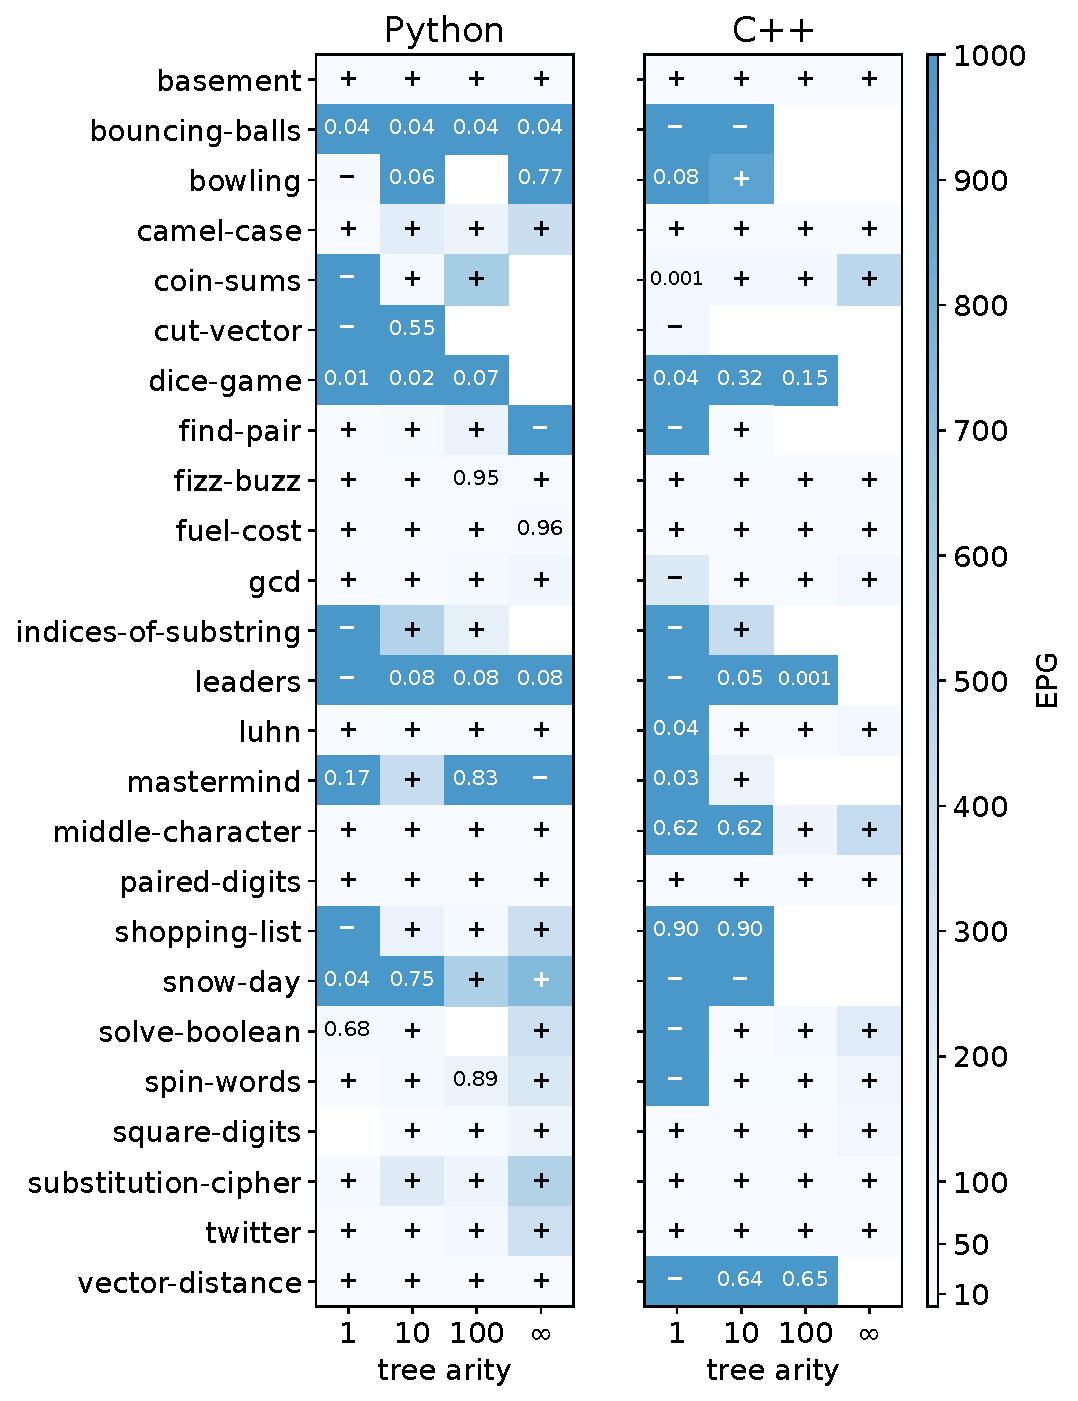
\includegraphics[width=.56\textwidth, trim={3mm 1.6mm 3mm 2mm}, clip]{img/seidr/results/num_programs_generated_vs_bf_test_pass_rate_vertical_maxprog_1000_v3.pdf}
  \caption{Number of excess programs generated (in color) and test pass rate (as numbers) depending on tree-arity. Higher EPG values are shown in darker shades than low EPG. We denote solved problems with ``+'' (test pass rate = 1), unsolved problems with ``-'' (test pass rate = 0), and show the test pass rate for partially solved problems. }
  \label{fig:seidr:epg-bf}
  %
  \vspace*{-3ex}
\end{figure*}
Out of 100 experiments for each language, in 21--24\% of runs in Python and C++, the draft program is already the solution (EPG=0). 
For 31--33\% of the experiments, the solution is found after discarding 5 candidates. 
Around half of the experiments do not generate more than 100 programs. 
However, 5 problems are solved with more than 500 generated programs in Python and 1 problem in C++ (with $N=10$).
The results imply that the first steps in the update of the draft program are crucial for solving the problem. 
The chances of solving the problem in later stages of the search, such as after 100 programs have been generated, are low.
This confirms our initial assumption in Section~\ref{sec:seidr-trade-off-settings} that 1000 programs are sufficient.

To briefly analyze Figure~\ref{fig:seidr:epg-bf}, we observe that some problems are solved in both languages, whereas some others --- only in Python. 
In addition, only five problems are not solved in any \method{} configuration in Python (bouncing-balls, bowling, cut-vector, dice-game and leaders) and seven in C++ (bouncing-balls, cut-vector, dice-game,  leaders, shopping-list, snow-day, and vector-distance).
Upon closer inspection of generated programs, we have noticed that in bouncing-balls, the programs have logical errors and differ considerably between programming languages, as well as in the majority of unsolved problems. 
Test cases and debug instructions in bowling frequently skewed the resulting programs to return answers to individual bowling score strings instead of writing an algorithm for calculating the score based on each next character.
The latter mistake happened in other unresolved problems, such as cut-vector.
Qualitative analysis has also shown that some programs failed to read input from the user and instead defined input strings within the code, which limited the program to test only one I/O pair, although the algorithm was correct.

% \begin{mdframed}[style=mystyle]
\begin{framed}
\noindent
\textbf{Repair-replace trade-off in the initial exploration (RQ1):} 
\method{} with Codex as the coding LLM outperforms the PushGP baseline on PSB2 in Python and performs on par with it in C++ experiments with tree-arity of 10. 
Search strategies with tree-arity larger than one benefit from the replace possibility of the \method{} framework as a consequence of using variable temperature for Codex-edit.
The repair component is also crucial for the framework because the replace-only search policy (with tree-arity of $\infty$) performs worse than the policies that alternate between replace and repair during program update (with tree-arity of 10 or 100).  
\end{framed} 
% \end{mdframed}


\subsubsection{Prompt Engineering in Initial Exploration}
We report the number of problems solved for different static and GPT-assisted debug instructions in Figure~\ref{fig:seidr:solved-vs-prompt-id}. 
Because debug instructions are part of the prompts for the LLMs and the program candidate format does not change, we will use the term prompt during the analysis of experiment results with different instructions.
Overall, the performance of the framework is robust to the debug prompt choice, both with LLM-generated and static templates. 
The number of solved problems differs for Python and C++ in our experiments.

\begin{figure}[tb]
  \centering
  \includegraphics[width=.7\linewidth, trim={0mm 2mm 0mm 2mm}, clip]{img/seidr/results/fig_7_num_solved_problems_vs_prompt_id_maxprog_5_v3_zenodo.pdf}
  \caption{Number of solved PSB2 problems depending on the instruction choice for the fixed tree-arity of 1.}
  \label{fig:seidr:solved-vs-prompt-id}
\end{figure}

For C++, all debug prompts except \ref{seidr:prompt-2} result in the same or higher performance than the instruction \ref{seidr:prompt-0} that is used in the repair-replace trade-off experiments. 
The debug instruction \ref{seidr:prompt-2} contains the verbs ``yield'' and ``ensure'' which are probably rarely used in code documentation. 
The best debug instruction for C++ is the LLM-assisted template \ref{seidr:prompt-6} containing the word ``obviously'', which should indicate the confidence of the author of the bug summary that GPT-3 should mimic during autocompletion.



\begin{figure*}[t]
  \centering
  % \includegraphics[width=.99\textwidth, trim={3mm 2mm 3mm 2mm}, clip]{img/seidr/results/fig_8_num_programs_generated_vs_propmt_id_test_pass_rate_vertical_maxprog_5_v3_zenodo.png}
  \includegraphics[width=.99\textwidth, trim={3mm 1.6mm 3mm 2mm}, clip]{img/seidr/results/fig_8_num_programs_generated_vs_propmt_id_test_pass_rate_vertical_maxprog_5_v3_telo.pdf}
  % % \vspace*{-2mm}
  \caption{Number of excess programs generated (in color) and test pass rate (as numbers) depending on the type of debug prompt. Higher EPG values are shown in darker shades than low EPG. We denote solved problems with ``+'' (test pass rate = 1), unsolved problems with ``-'' (test pass rate = 0), and show the test pass rate for partially solved problems. }
  \label{fig:seidr:epg-prompt-test}
  %
  \vspace*{-3ex}
\end{figure*}

Python programs do not show the same effect during experiments with different prompts. 
The overall performance drops in comparison with using the prompt \ref{seidr:prompt-0}. 
By limiting the total number of generated programs from 1000 
to 5 in the current set of experiments, we lose 2 problem solutions in Python with \ref{seidr:prompt-0}. 
The prompt that results in the best performance in C++ for the EPG limit of 5 corresponds to the worst performance in Python. 
This result can occur due to the small tree-arity and low variability of debugging updates of the initial draft. 
Another reason is that the GPT summary of bugs may not point to logical errors. The model for text autocompletion frequently outputs bug summaries that mention ``the code is not accepting the input correctly.''
Note that such bug summary appears in other debug prompts, too. 

To analyze the effect of using different prompts at a problem level, we present a heatmap of EPG for all 25 problems in Figure~\ref{fig:seidr:epg-prompt-test}. 
We add the values of test pass rate in numbers or signs and show EPG in color. 
Empty cells denote that the search halts due to other OpenAI exceptions, such as \texttt{APIError}.\footnote{~\url{https://platform.openai.com/docs/guides/error-codes/python-library-error-types}}
\ag{In addition, if the framework halts before max programs attempts (light-blue cells with a~``-''), it is due to the input length limit of underlying LLMs, i.e., the generated code is too long and does not fit as input to the LLM.}

Some problems are solved with all prompts, while other problems are solved with only a subset of prompts, solved partially, or not solved at all. 
A number of problems are solved with all or the majority of prompts in both languages, such as basement, fizz-buzz, paired-digits, and twitter.
Other problems pass all tests in only one of the languages, such as luhn, vector-distance, fuel-cost, or substitution-cipher. 
Most of the solved problems are generated as the first draft or within 1--2 debug steps. 
However, some problems pass 90\% of test cases at the fifth step, such as substitution-cipher in Python with prompts \ref{seidr:prompt-4} and \ref{seidr:prompt-8} or shopping-list in C++ with prompts \ref{seidr:prompt-0}, \ref{seidr:prompt-1}, \ref{seidr:prompt-5} and \ref{seidr:prompt-7}. 
These runs are likely to be updated with the fully correct programs in the following several steps, according to the results in Section 5.1, but the experiments
are stopped for the fairness of inter-prompt comparison.
\ag{Alternatively, conducting the prompt engineering experiment with 1000 max programs would have shown what prompts are beneficial for solving the problems in the long run and can be interesting for future work.}

The most interesting cases concern the problems that are solved only with LLM bug summary or only with static prompts, depending on how well the LLM can pick up the bug and explain it to Codex. 
For example, the gcd problem is solved only with prompts \ref{seidr:prompt-6}--\ref{seidr:prompt-10} in C++ and is not solved with either of \ref{seidr:prompt-0}--\ref{seidr:prompt-5}. 
A similar result is obtained for spin-words and coin-sums in C++.
In Python, we observe only the cases where solutions are obtained with static prompts and are not obtained with GPT-assisted prompts, e.g., for find-pair, camel-case. In addition, several prompts work well from both S and M categories as for gcd. 


\begin{framed}
\textbf{Prompt engineering in the initial exploration (RQ2):} 
Program synthesis in C++ with \method{} achieves better performance in the repair-only setting with both GPT-assisted prompts that summarize bugs in code and static templates that describe failing I/O cases. 
The best-performing C++ instruction is obtained with GPT for text completion that contains the word ``obviously.''
Results for PSB2 solutions in Python differ: the static prompt template \ref{seidr:prompt-0} results in the best performance. 
Overall, \method{} performance is stable with different debugging prompts submitted to Codex-edit.
\end{framed}


\subsection{Generalizability Experiments}

In this section, we present and discuss replace-repair trade-off results obtained with GPT-3.5 and Llama 3 and the effect of switching from tournament selection to lexicase selection for the best hyperparameter settings found for the trade-off. 
We count the number of fully solved problems as measured by $TPR=1$ in experiments with the hyperparameter settings described in Table~\ref{tab:w-n-generalizability} in 6 runs and present the language-specific results for PSB2 and HumanEval.
% in Figure~\ref{fig:repair-replace-trade-off-generalizability}. 
We also explore the distribution of the average speed of obtaining solutions 
% in Figure~\ref{fig:epg-distribution} 
and in how many of the 6 runs each problem is fully solved (i.e., reached $TPR=1$).
% in Figures~\ref{fig:epg-num-solved-psb2},~\ref{fig:epg-num-solved-he-python}, and~\ref{fig:epg-num-solved-he-c++}. 
The figures are described in detail in the dedicated sections. 

\subsubsection{Repair-replace Trade-off and Robustness to Restarts in the Generalizability Experiments.}
\label{sec:seidr-treearity-ollama}\label{sec:seidr-results-rq3}

We compare the number of solved problems in the experiments with $\treearitydraft{}=\treearitydebug{}$ values of 1, 2, 4, 10, 16, $\infty$ (100) and $\treearityexplain{}=2$ in Python and C++ in Figure~\ref{fig:repair-replace-trade-off-generalizability}. 
We will refer to the (equally set) values of $\treearitydraft{}$ and $\treearitydebug{}$ as $N^*$ further in the text.
As previously, the experiments with $N^*=1$ and $N^*=\infty$ correspond to ablation studies, where the replace option or repair option is turned off. 
The results of \method{} are compared to the baseline performance of PushGP on the PSB2 benchmark, which solves 17 out of 25 problems. 
The boxplots show the inter-quartile range between the first and third quartiles observed in 6 runs and the median values as horizontal lines within the boxes. 

%%%%%%%%%%%%%%%%%%%%%%%%%%%%%%%%%%%%%%%%%%
% Num solved problems
%%%%%%%%%%%%%%%%%%%%%%%%%%%%%%%%%%%%%%%%%%
\begin{figure}[bt]
\begin{subfigure}{\linewidth}
\centering
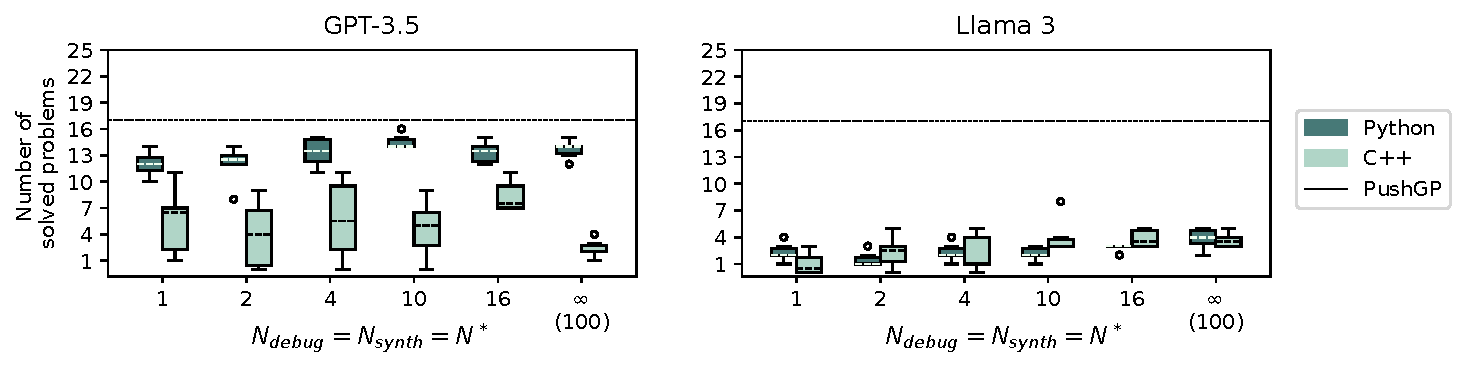
\includegraphics[width=\linewidth, trim={0mm 0mm 0mm 0mm}]{img/results/num_solved/num_solved_problem_psb2_6runs_boxplot_v5.pdf}
\vspace{-15pt}
  \caption{PSB2}
  \label{fig:num-solved-psb2-gpt3.5}
\end{subfigure}
\begin{subfigure}{\columnwidth}
\centering
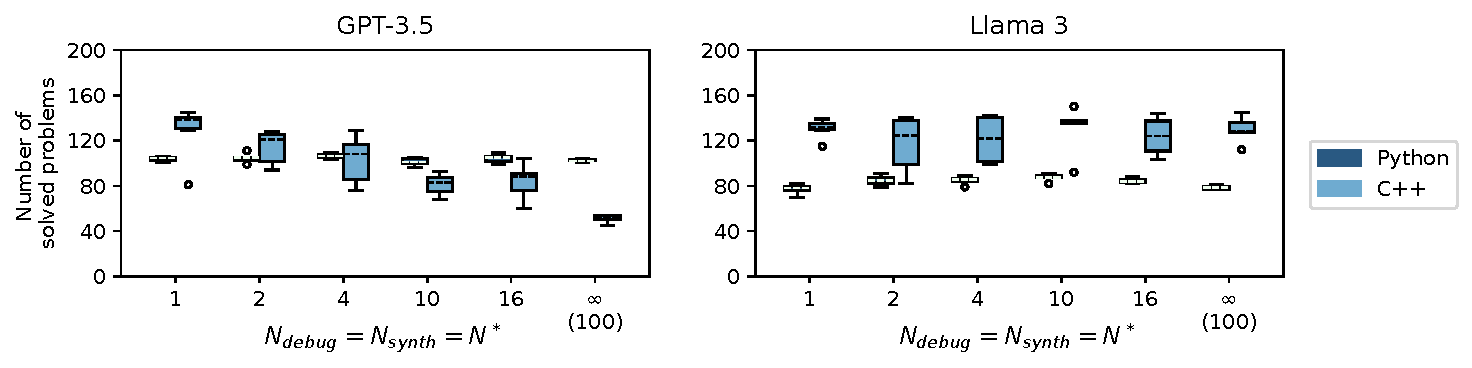
\includegraphics[width=\linewidth, trim={0mm 0mm 0mm 0mm}]{img/results/num_solved/num_solved_problem_humaneval_6runs_boxplot_v5.pdf}
\vspace{-15pt}
  \caption{HumanEval}
  \label{fig:num-solved-he-gpt3.5}
\end{subfigure}
\vspace{-16pt}
\caption{Repair-replace trade-off as a tree search problem in \method{}: the total number of solved problems as measured by $TPR=1$ using \method{} with GPT-3.5 and Llama 3 depending on tree-arity $N^*$.}
% \vspace{2pt}
\label{fig:repair-replace-trade-off-generalizability}
\end{figure}


The trend present for all the datasets and models is that the results for Python are more condensed over 6 runs than for C++. 
Since access to statistics about the training data for Llama 3 and GPT-3.5 is not provided, reasons for more stable performance in Python across runs can possibly lie in the training data distribution but cannot be confirmed. 
However, the fact that HumanEval-Python is a popular code generation benchmark, against which models are compared, may affect the results on this and other Python benchmarks.
In the same line of comparison of the results between two programming languages, \method{} with \gpt{} performs better in \py{} than in \cpp{} on PSB2. 

% In the majority of experiments, based on the number of fully solved problems, it is beneficial to use the tree-arity larger than 1 and less than $\infty, $ except for \gpt{} on HumanEval-C++. 
% This result confirms that, for the majority of cases, using \method{} that builds a tree of solutions is better than repairing only one program or regenerating the program from scratch every time. 
% 
\llama{} performs worse than \gpt{} on PSB2 in both languages.
This dataset has more test cases in stock than HumanEval and can be considered a more thorough test of the coding and debugging capabilities of LLMs. 
Following a recent trend, where larger models outperform the smaller ones, the results of \method{} on PSB2 confirm that the smaller model (\llama{}) performs worse than the larger one (\gpt{}).

Looking back at the initial experiments with Codex and PSB2, we notice the degradation of performance from Codex to GPT-3.5: \method{} with Codex solved 19 problems in Python and 17 in C++ with tree-arity 10, while the best-performing result of \method{} GPT-3.5 is 16 (tree-arity of 10, too) in Python and 11 in C++ (several tree arities, but not 10). 
This result can be explained by the focus of LLM builders on generalization of knowledge and performance on a variety of tasks, while Codex specializes on code generation.
Moreover, due to increased costs from Codex to GPT-3.5, we decrease the number of maximum generated program candidates from 1000 for Codex to 100 for GPT-3.5. 
However, only two problems are solved with Codex with $EPG > 100$: indices of substring (at program candidate \#510) and substitution cipher (at candidate \#210) in Python, bowling (candidate \#912) and indices of substring (\#410) in C++. 
In the meantime, some problems are solved by Codex earlier than at the debugging attempt \#100 and not solved by GPT-3.5 and vice versa. 
Therefore, reduction of the maximum generated programs has only a partial effect on the difference between results of two models. 


\begin{figure}[bt]
\begin{subfigure}{\linewidth}
\centering
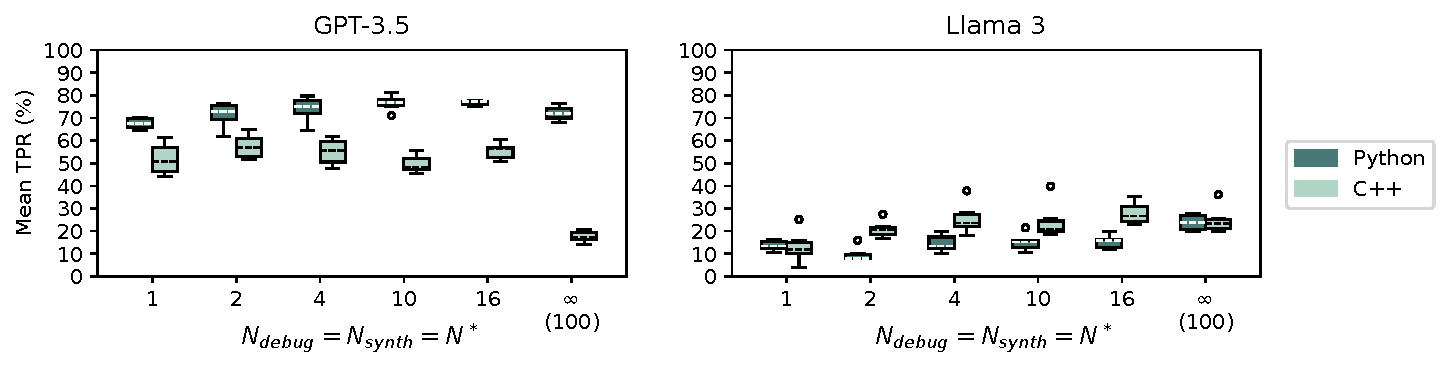
\includegraphics[width=\linewidth, trim={0mm 0mm 0mm 0mm}]{img/results/mean_tpr/mean_tpr_psb2_6runs_boxplot_v5.pdf}
\vspace{-15pt}
  \caption{PSB2}
  \label{fig:mean-tpr-psb2-gpt3.5}
\end{subfigure}
\begin{subfigure}{\columnwidth}
\centering
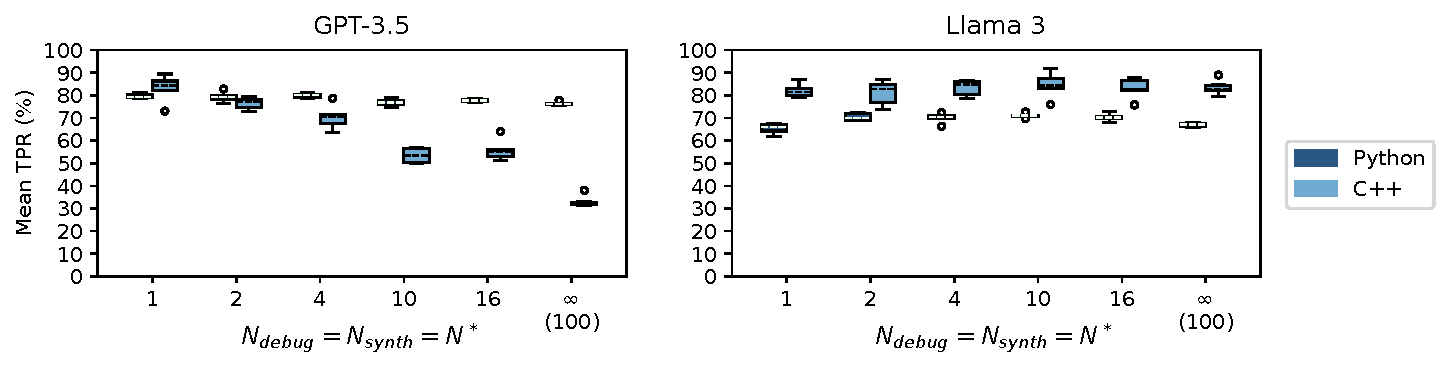
\includegraphics[width=\linewidth, trim={0mm 0mm 0mm 0mm}]{img/results/mean_tpr/mean_tpr_humaneval_6runs_boxplot_v5.pdf}
\vspace{-15pt}
  \caption{HumanEval}
  \label{fig:mean-tpr-he-gpt3.5}
\end{subfigure}
\vspace{-16pt}
\caption{Repair-replace trade-off as a tree search problem in \method{}: mean $TPR$ measured in \% obtained using \method{} with GPT-3.5 and Llama 3 depending on tree-arity $N^*$.}
\label{fig:mean-tpr-repair-replace-trade-off-generalizability}
\end{figure}


In addition to reporting the number of fully solved problems, we also report mean Test Pass Rate measured in \% in Figure~\ref{fig:mean-tpr-repair-replace-trade-off-generalizability}. 
For HumanEval-C++, \method{} with \gpt{} has better results with smaller tree-arity values than with larger ones.
In Python, experiments with $1 < N^* < 100$ (i.e., non-corner case values of $N^*$) yield better mean TPR for \method{} with \gpt{} on PSB2 and with \llama{} --- for HumanEval-Python.
\method{} with \llama{} performs with slightly better mean TPR towards larger $N^*$  on PSB2-C++, and at the same time, it performs well on HumanEval-C++, so the difference between results with different $N^*$ is small.
The maximum of mean TPR for both datasets and models and max number of solved problems are obtained with $N^*=16$ or less, except for Llama 3 in PSB2-C++. 
From this part of experiments, we notice that moderate or small tree arities $(N^* \le 16)$ are preferred, but there is no one leading tree-arity.


The number of runs in which a problem is solved and the average speed of finding those solutions are shown in Figure~\ref{fig:epg-num-solved-psb2} for PSB2, Figure~\ref{fig:epg-num-solved-he-python}
for HumanEval-Python and Figure~\ref{fig:epg-num-solved-he-c++} for HumanEval-C++.
These figures show what problems were not solved in any run of any experiment (a row with zeros colored white) and what problems are easier to solve than others (e.g., solved in 6 out of 6 runs, or at least one with each tree-arity $N^*,$ or earlier in the search tree and shown in brighter rather than darker color but not white). 
We also show the results of lexicase selection runs marked with ``lex.'' in these three figures but discuss them in a separate section. 

The majority of solved PSB2 problems are solved in more than one run per setting with \gpt{} and faster (with fewer attempts) in Python than in C++ as illustrated in Figure~\ref{fig:epg-num-solved-psb2}.
For \llama{}, most of the solutions are obtained in 1--3 runs.
The trend for both  datasets is that, for the problems where a solution is found, \method{} with \gpt{} makes fewer attempts in Python (brighter colors prevail in the corresponding parts of Figures~\ref{fig:epg-num-solved-psb2} and~\ref{fig:epg-num-solved-he-python}) than \method{} with \gpt{} in C++ or \method{} with \llama{} in both languages (darker shades in the \gpt{} on C++ and \llama{} parts of Figures~\ref{fig:epg-num-solved-psb2} and \ref{fig:epg-num-solved-he-c++}).


\begin{figure}[tb]
  \centering
  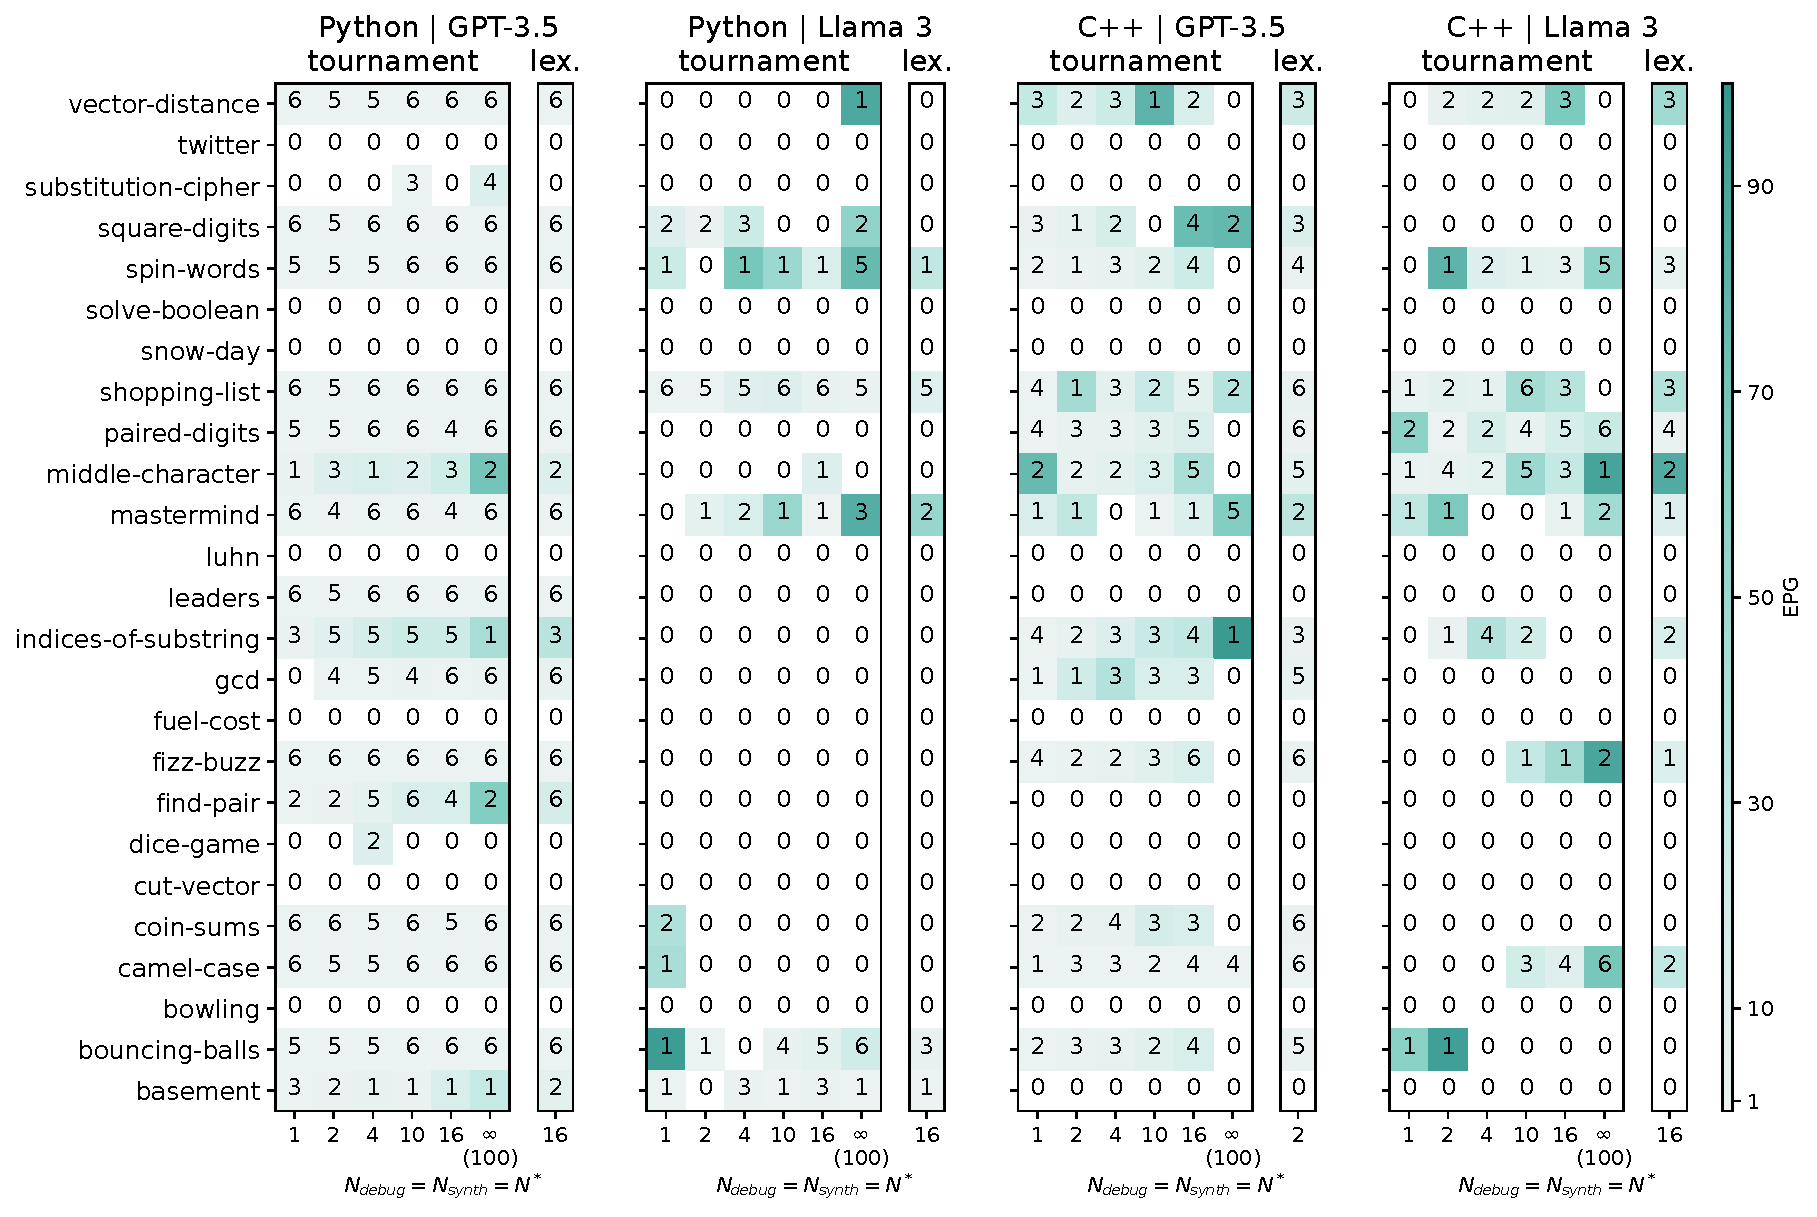
\includegraphics[width=\linewidth, trim={3mm 2.8mm 3mm 2mm}, clip]{img/results/solved_in_runs/epg_mean_and_num_runs_problem_solved_avg_score_check_w_lexicase_psb2_6runs_heatmap_v5.pdf}
  \caption{PSB2: mean Excess Programs Generated (in color) and the number of runs in which a task is solved. The experiments in which a specific problem is not solved in any run are shown in white.
  }
  \label{fig:epg-num-solved-psb2}
  \vspace{-3ex}
\end{figure}

\begin{figure}[hbt!]
  \centering
  % {left bottom right top},
  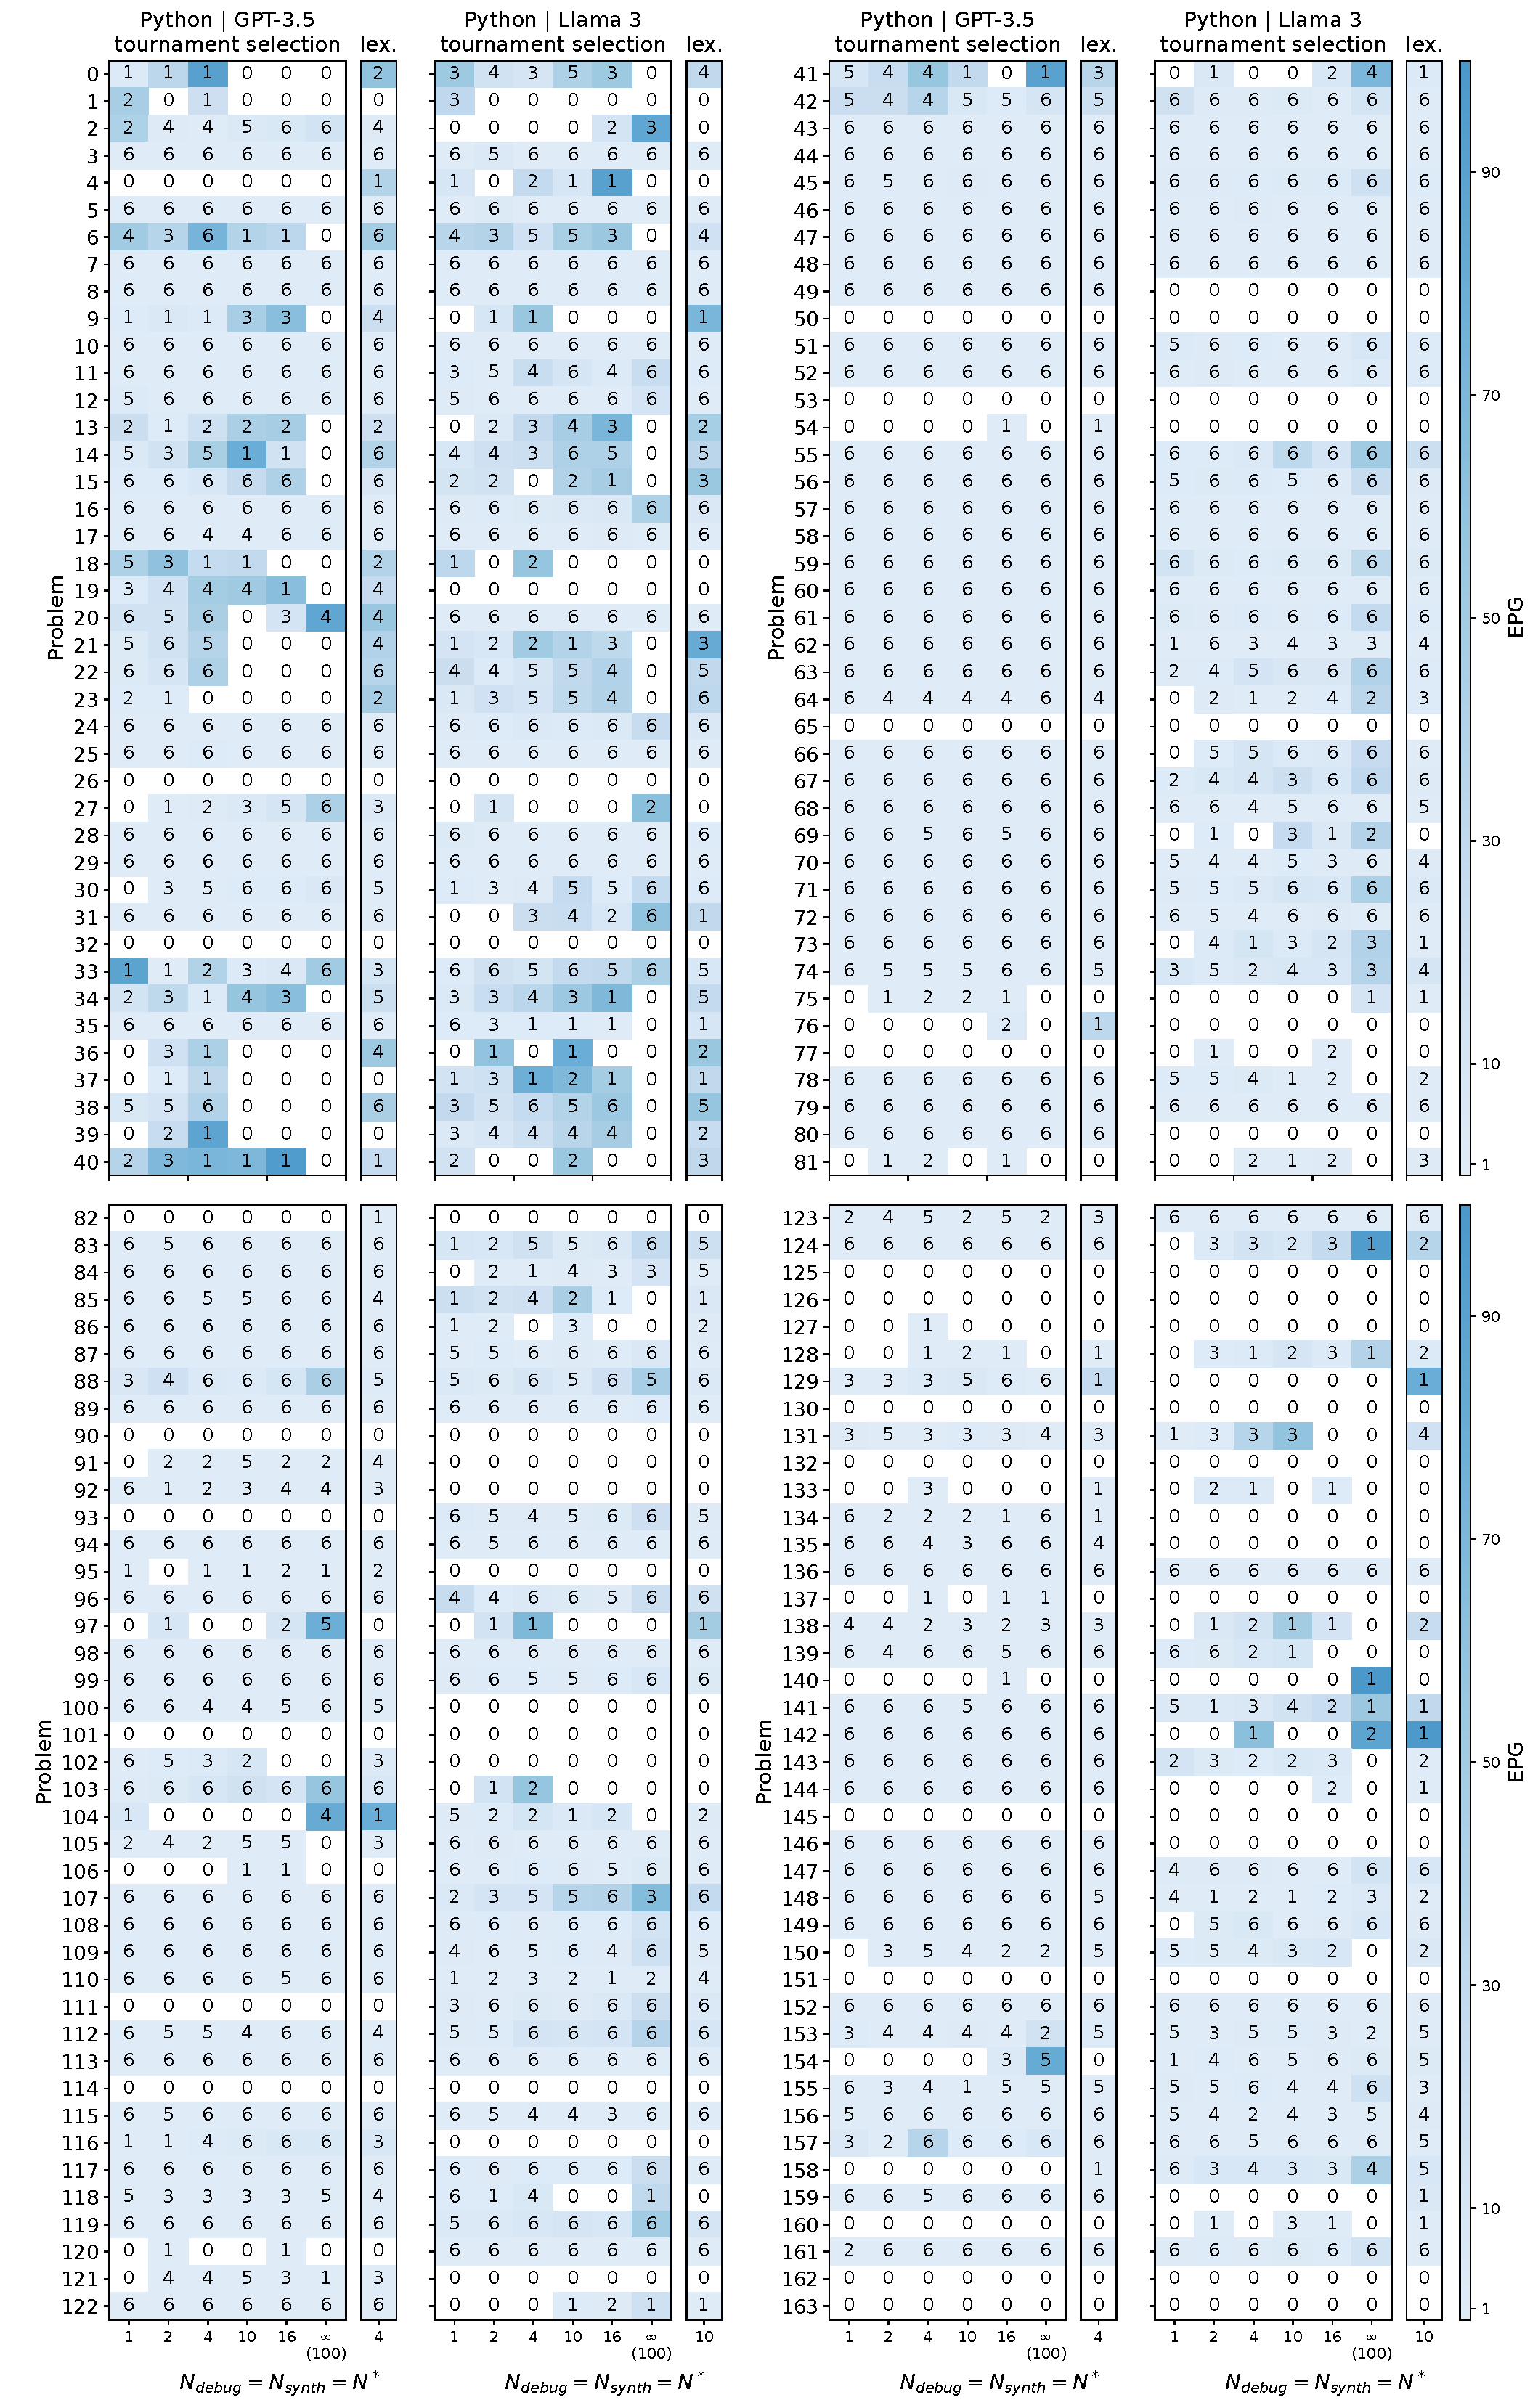
\includegraphics[width=.88\linewidth, trim={0mm 3mm 0mm 2.6mm}, clip]{img/results/solved_in_runs/epg_mean_and_num_runs_problem_solved_avg_score_check_w_lexicase_humaneval_Python_6runs_heatmap_v5.pdf}
  \vspace{-6pt}
  \caption{HumanEval-Python: mean Excess Programs Generated (in color) and the number of runs in which a task is solved. The problems that are not solved in any run are colored white.}
  \label{fig:epg-num-solved-he-python}
  \vspace{-10pt}
\end{figure}

\begin{figure}[hbt!]
  \centering
  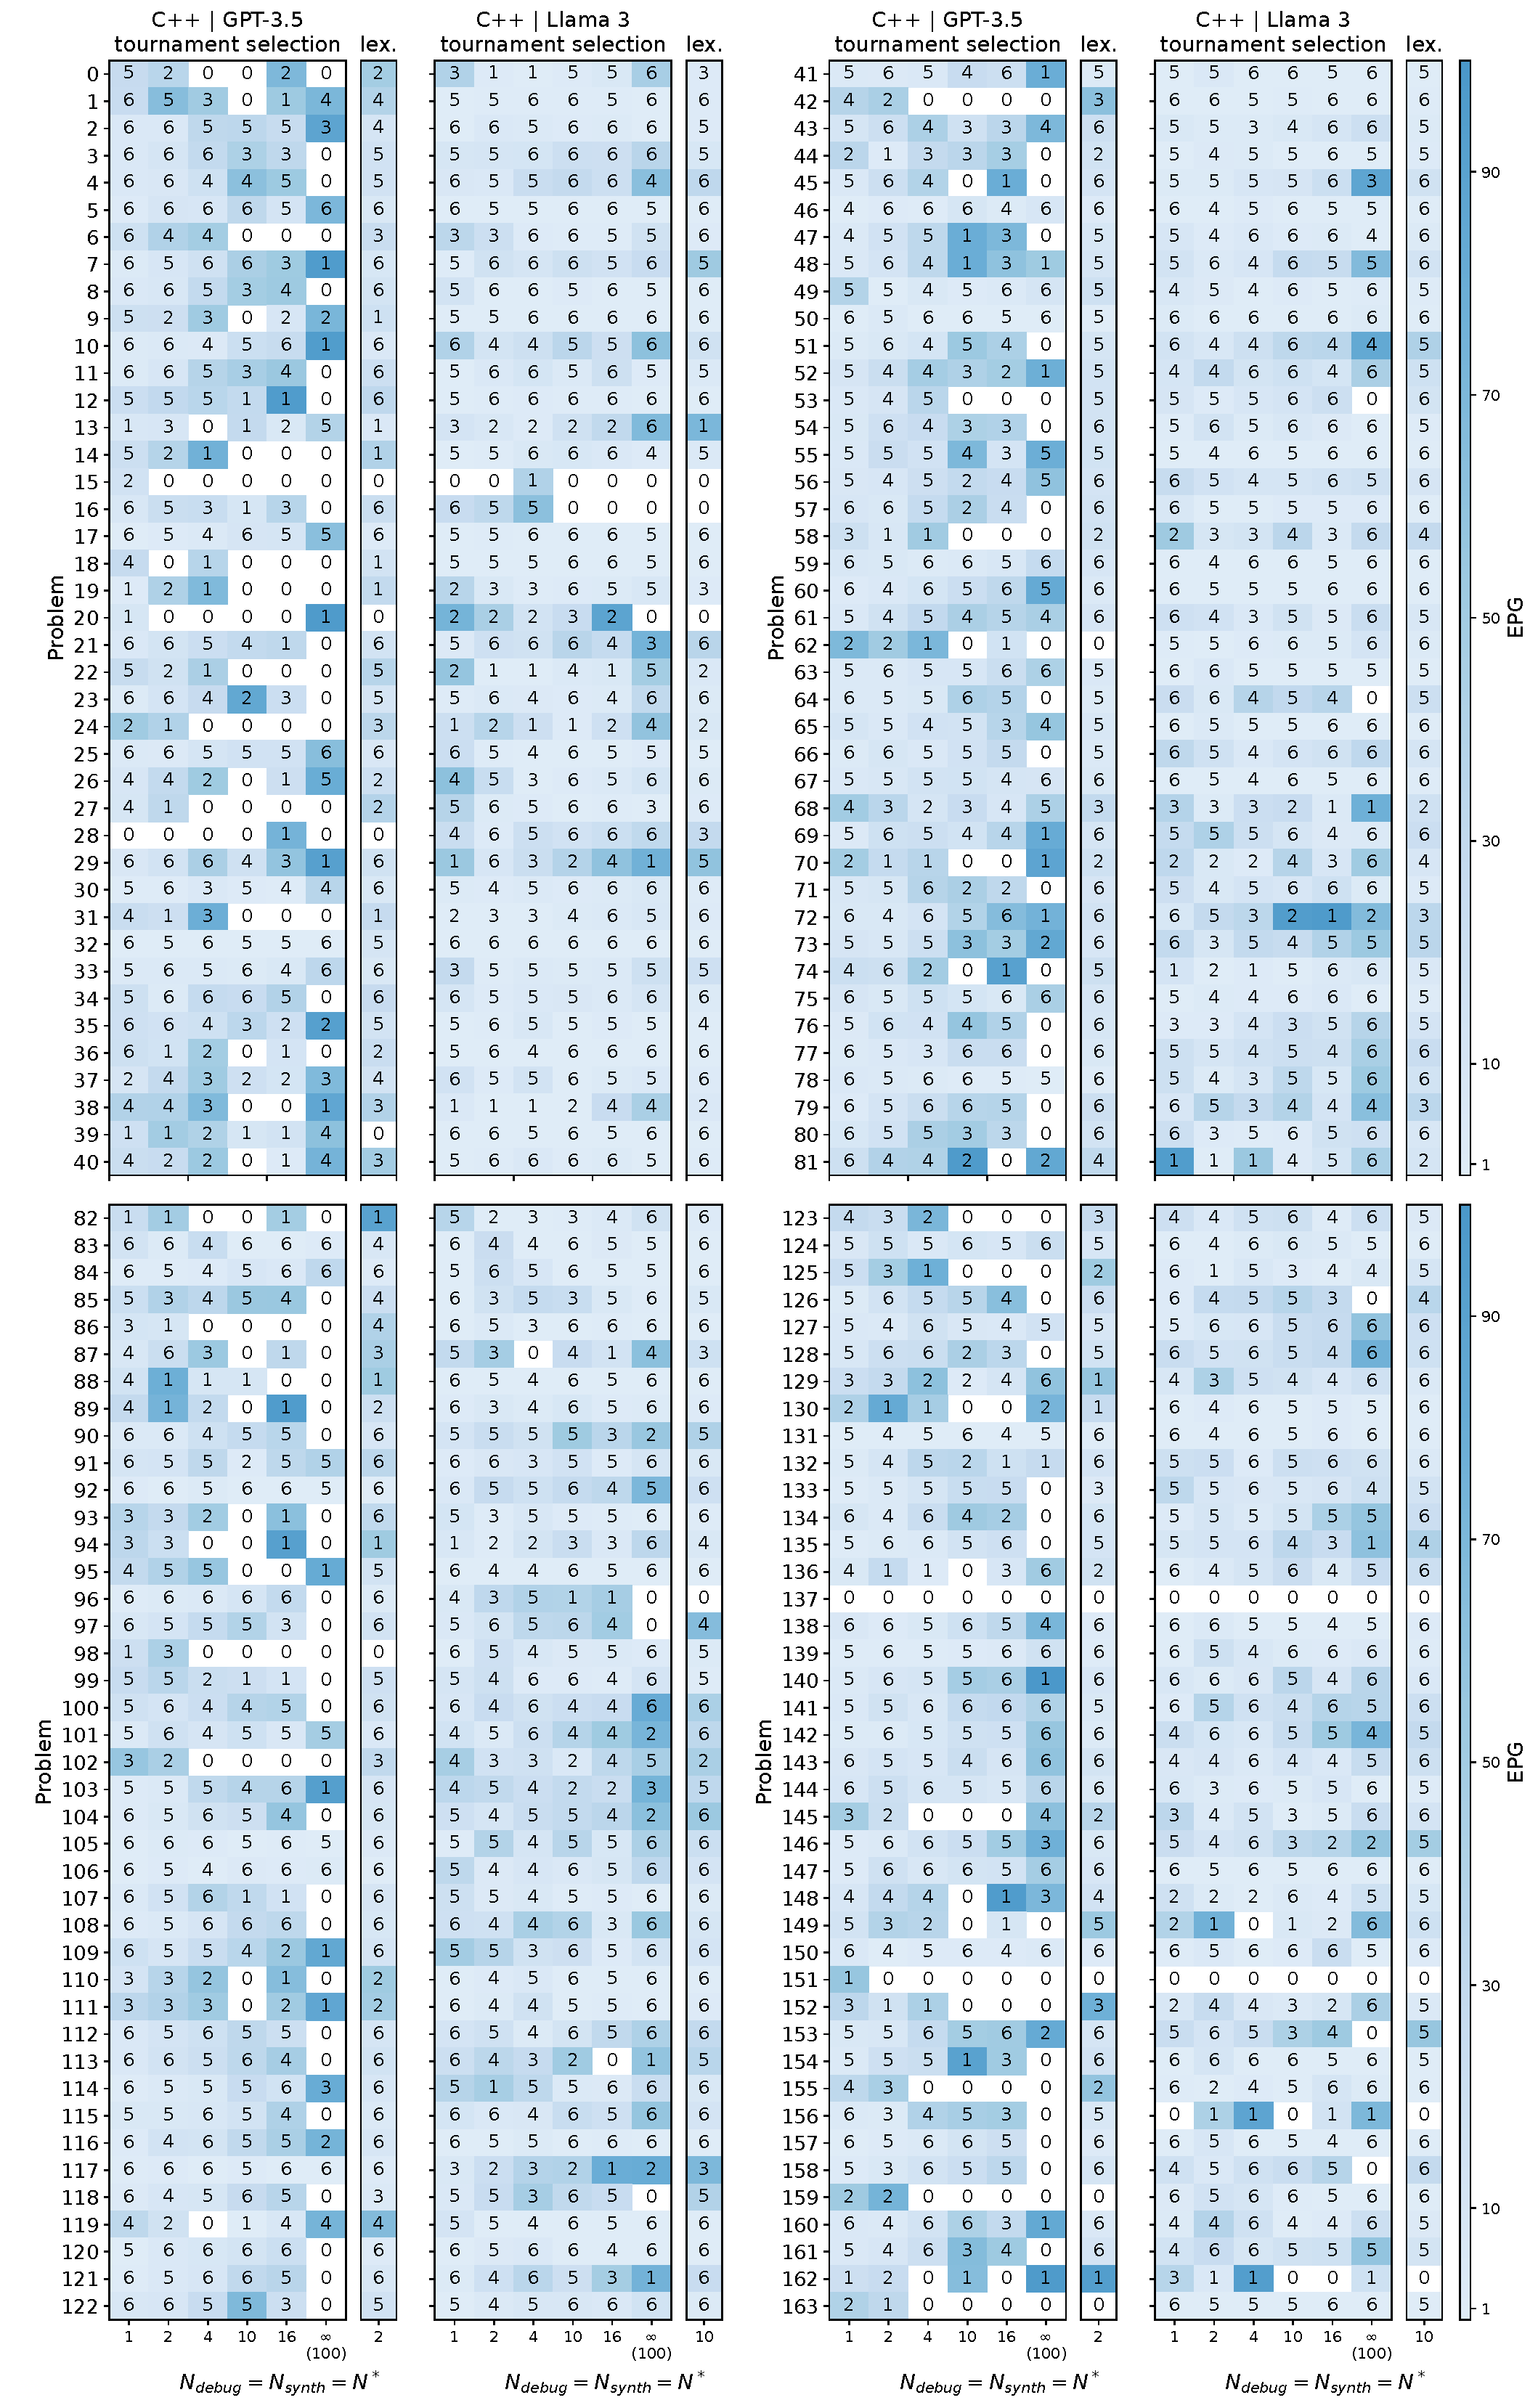
\includegraphics[width=.88\linewidth, trim={0mm 3mm 0mm 2.6mm}, clip]{img/results/solved_in_runs/epg_mean_and_num_runs_problem_solved_avg_score_check_w_lexicase_humaneval_C++_6runs_heatmap_v5.pdf}  %
  \vspace{-6pt}
  \caption{HumanEval-C++: mean Excess Programs Generated (in color) and the number of runs in which a task is solved. The problems that are not solved in any run are colored white.}
  \label{fig:epg-num-solved-he-c++}
  \vspace{-10pt}
\end{figure}


Given the resource constraints, such as costs of calling \gpt{} and the time of running each experiment, we limit restarts to 6 runs in total with each set of hyperparameters.
However, to explore the capabilities of \method{} with the studied models, we can take a union over experiments and count the number of problems solved at least once across 36\footnote{~We have 6 runs and 6 different values of $N^*.$} restarts with a fixed dataset, language and model.

In this way, in addition to reporting the number of problems solved in each run in the boxplot, we can derive the number of problems solved in any run with any set of hyperparameter using information in Figures~\ref{fig:epg-num-solved-psb2}--\ref{fig:epg-num-solved-he-c++}.
For example, \method{} with \gpt{} does not solve only 7 problems out of 25 PSB2-Python tasks (see Figure~\ref{fig:epg-num-solved-psb2}).
Namely, bouncing-balls, cut-vector, dice-game, indices-of-substring, middle-character, solve-boolean, and substitution-cipher are solved in 0 runs with all the variations of $N^*=N_{synth}=N_{debug}.$
In other words, 18 unique problems are solved in the collection of all the experiments using \method{} with \gpt{} on PSB2-Python. 
\method{} with \gpt{} does not solve 12 out of 25 PSB2-C++ tasks with any hyperparameter settings. 
The number of solved problems in any run with \method{} and \llama{} are 10 for PSB2 in both languages. 
To support the finding about degradation of performance happening in a non-specialized model GPT-3.5 compared to the code-specialized Codex, we calculate the number of solved problems in any run with Codex and obtain 20 problems solved at least once in Python and 18 in C++. 

Similarly, \method{} with \gpt{} solves 141 out of 164 HumanEval-Python problems at least once in all runs, collectively, and 128 problems with \llama{} (see Figure~\ref{fig:epg-num-solved-he-python}).
In HumanEval-C++, \method{} with \gpt{} solves 163 out of 164 problems (except CPP/137) in the union of all runs and 162 with \llama{} (except CPP/137 and CPP/151) as follows from Figure~\ref{fig:epg-num-solved-he-c++}.


In Figure~\ref{fig:epg-distribution}, we present the analogy of the speed of obtaining solutions, EPG. 
We zoom in to the cases with solutions found with up to the first 10 program candidates in Figures~\ref{fig:psb2-epg-distrib-step-1} and~\ref{fig:humaneval-epg-distrib-step-1} for PSB2 and HumanEval-X, respectively. 
The coarser-grained EPG distribution with the step of 10 candidates is shown in Figures~\ref{fig:psb2-epg-distrib-step-10} and~\ref{fig:humaneval-epg-distrib-step-10}. 


% %%%%%%%%%%%%%%%%%%%%%%%%%%%%%%%%%%%%%%%%%%
% % EPG distribution
% %%%%%%%%%%%%%%%%%%%%%%%%%%%%%%%%%%%%%%%%%%
\begin{figure}[tb]
\vspace{-2.2ex}
\begin{subfigure}{.8\columnwidth}
\centering
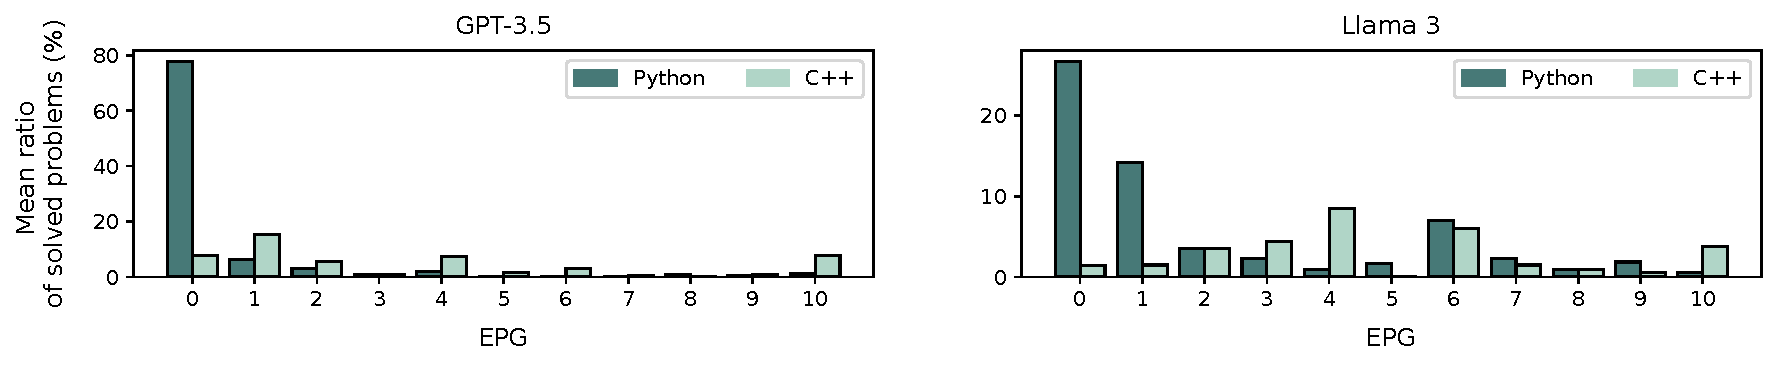
\includegraphics[width=\linewidth, trim={0mm 4mm 0mm 0mm}, clip]{img/results/epg_distribution/epg_distribution_step_1_psb2_6runs_barplot_v5.pdf}
  \caption{PSB2: 0 $\leq$ EPG $\leq$ 10 with step 1.}
  \label{fig:psb2-epg-distrib-step-1}
\end{subfigure}
% 
% 
\begin{subfigure}{.8\columnwidth}
\centering
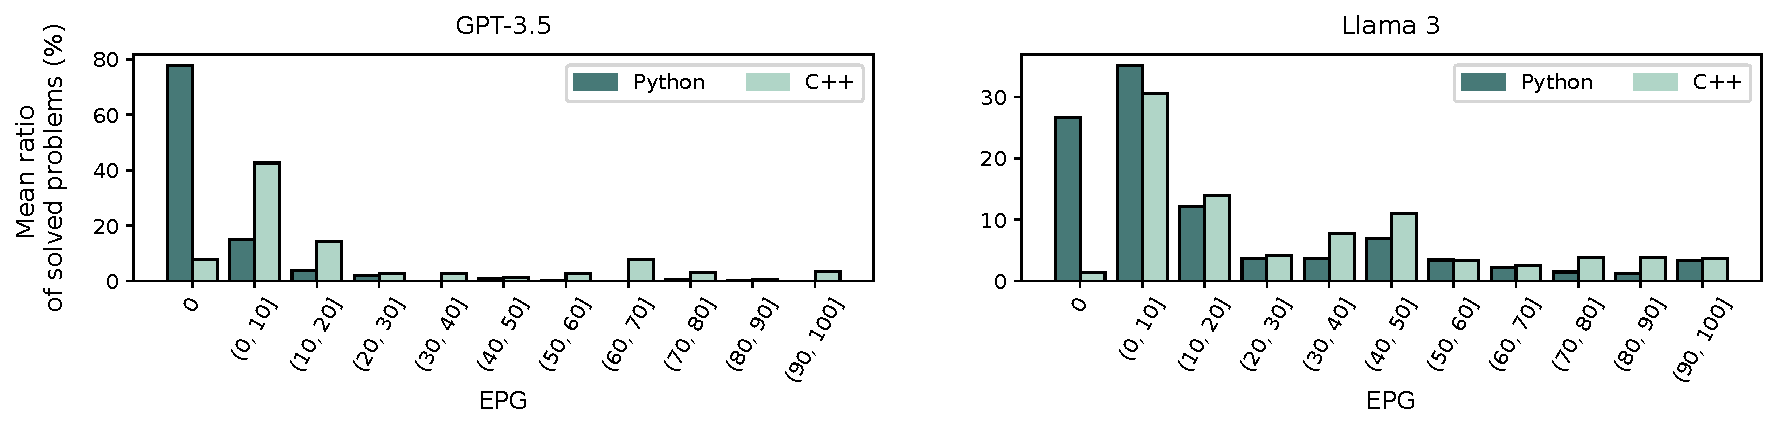
\includegraphics[width=\linewidth, trim={0mm 4mm 0mm 0mm}, clip]{img/results/epg_distribution/epg_distribution_step_10_psb2_6runs_barplot_v5.pdf}
  \caption{PSB2: 0 $\leq$ EPG $\leq$ 100 with step 10.}
  \label{fig:psb2-epg-distrib-step-10}
\end{subfigure}
% 
\begin{subfigure}{.8\columnwidth}
\centering
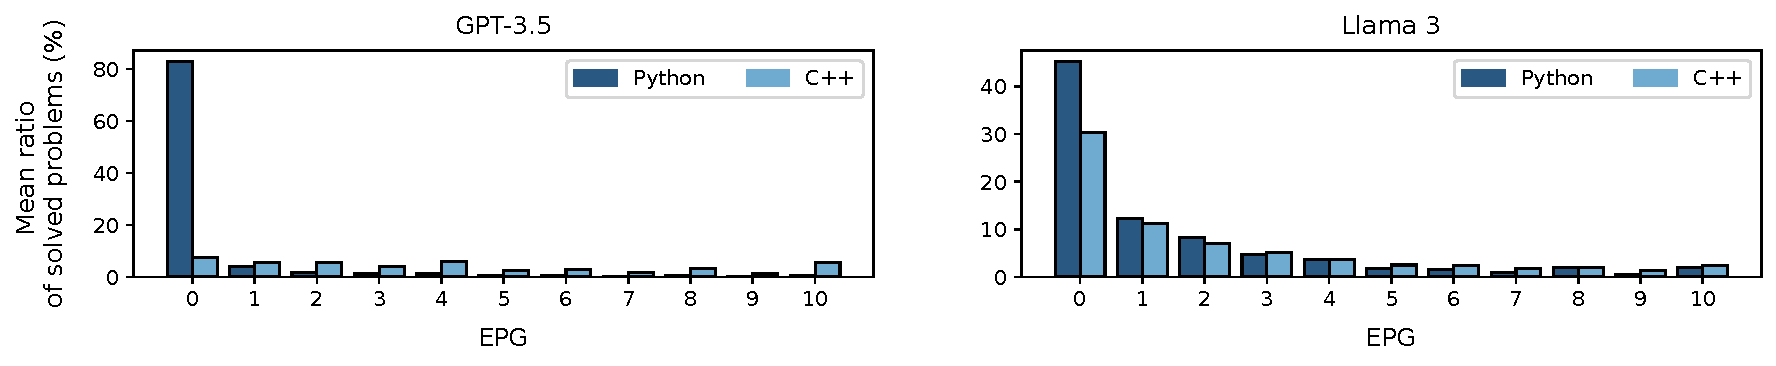
\includegraphics[width=\linewidth, trim={0mm 4mm 0mm 0mm}, clip]{img/results/epg_distribution/epg_distribution_step_1_humaneval_6runs_barplot_v5.pdf}
  \caption{HumanEval: 0 $\leq$ EPG $\leq$ 10 with step 1.}
  \label{fig:humaneval-epg-distrib-step-1}
\end{subfigure}
% 
\begin{subfigure}{.8\columnwidth}
\centering
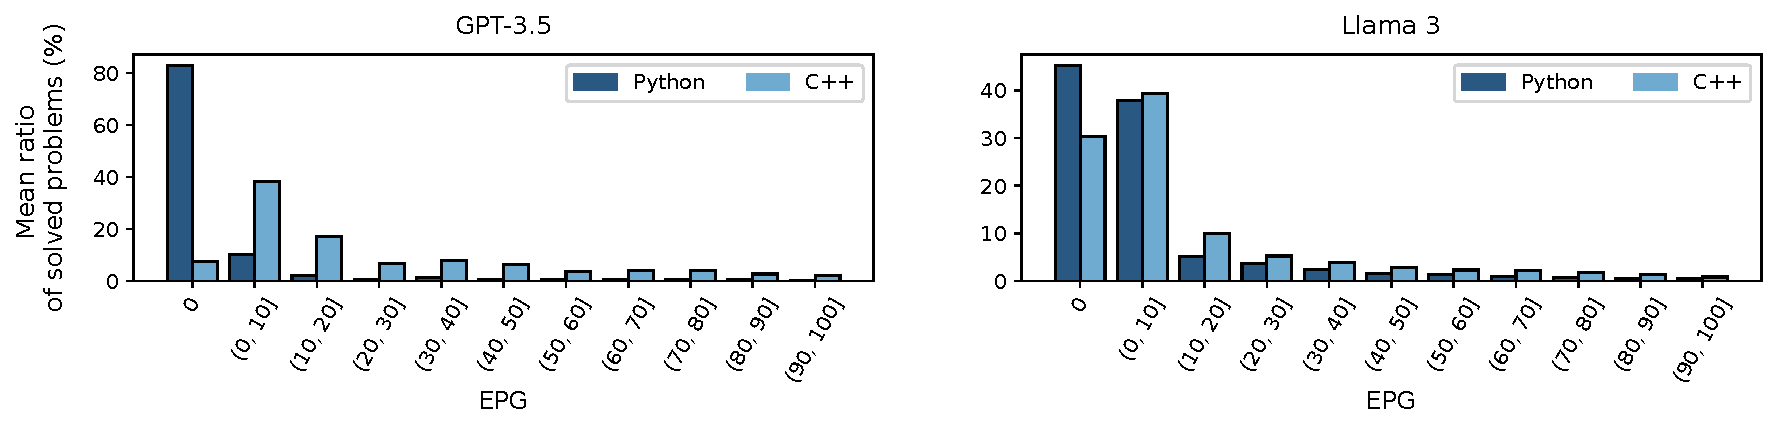
\includegraphics[width=\linewidth, trim={0mm 4mm 0mm 0mm}, clip]{img/results/epg_distribution/epg_distribution_step_10_humaneval_6runs_barplot_v5.pdf}
  \caption{HumanEval: 0 $\leq$ EPG $\leq$ 100 with step 10.}
  \label{fig:humaneval-epg-distrib-step-10}
\end{subfigure}
\vspace{-10pt}
\caption{Distribution (in \%) of the number of generated programs with GPT-3.5 and Llama 3 during each problem-solving attempt on average over 6 runs with different tree arities $\treearitydraft{}, \; \treearitydebug{}.$}
\label{fig:epg-distribution}
\vspace{-3ex}
\end{figure}



In detail, we show the distribution of EPG values in all experiments to explore what proportion of candidate updates is made before the solution is found.
For example, on average, over 70\% of Python solutions by \method{} with \gpt{} are solved from the first attempt, i.e., have EPG$=0$ (see Figure~\ref{fig:psb2-epg-distrib-step-1}).
Python solutions are more frequently found from the first attempt by \method{} with \llama{} than later in the tree, although less frequently than with \gpt{}.
Most of solutions found by \method{} benefit from the iterative repair and generate up to 10 extra programs with both models (see Figures~\ref{fig:psb2-epg-distrib-step-10}, \ref{fig:humaneval-epg-distrib-step-10}). 
However, some solutions are also found later in the tree search. 

The EPG distribution results for correctly solved problems with $TPR=1$ imply that the first steps in the update of the draft program are crucial for solving the problem. 
The chances of solving the problem in the later stages of the search are low.
This confirms our assumption in Section~\ref{sec:seidr-trade-off-settings} that 100 programs are sufficient in the generalizability experiments.

\begin{framed}
\textbf{Repair-replace trade-off for \method{} with GPT-3.5 and \llama{} in the generalizability experiments (RQ1, RQ3, RQ4):}

Unlike for \method{} with Codex and a fixed debugging instruction (see Section~\ref{sec:seidr-seidr:rq1}), \method{} with \gpt{} and \llama{} does not show any distinct trend for all the languages and datasets in terms of the preferred tree-arity value. 
Results over a number of runs with the same hyperparameter settings are more condensed for Python than for C++, which can be a result of optimizing LLMs for high performance on popular coding benchmarks in Python.
If solutions to problems are found by \method{}, it is done at an earlier tree search step for Python than for C++ (i.e., with a smaller EPG). 
The majority of solutions are found within the first 10 updates of program candidates. 
\method{} solves 163 out of 164 HumanEval-C++ problems with \gpt{} at least once over all runs with all restarts and hyperparameter sets, and 162 --- with \llama{}.
\end{framed}



\subsubsection{Parent Selection Strategies within the Ranking Agent in the Generalizability Experiments}
\label{sec:seidr-lexicase-results}

Based on the mean TPR over all runs reported in Figure~\ref{fig:mean-tpr-repair-replace-trade-off-generalizability}, we fix the best-performing $N^*$ for each dataset, language and model and run the experiments with lexicase selection instead of tournament selection as a parent selection strategy. 
The hyperparameters are shown in Table~\ref{tab:lexicase-selection-hyperparameters}.
We compare the number of problems solved  with these settings and two types of parent selection algorithms in Figure~\ref{fig:num-solved-lexicase-selection} and mean TPR in Figure~\ref{fig:mean-tpr-lexicase-selection}.
Mean TPR with lexicase selection and the best tournament selection configuration are similar for two selection strategies for most of the experiments.
Similar results are obtained for the number of fully solved problems, with the exception of C++ results of \method{} with \gpt{} on both datasets, where lexicase selection improved the results.

\begin{table}[t]
\vspace{-2.6ex}
\setlength{\tabcolsep}{4pt}
\centering
\caption{\method{} generalizability experiments: hyperparameters in the lexicase selection experiments.}\small
\label{tab:lexicase-selection-hyperparameters}
\begin{tabular}{rcccc|cccc}
\toprule
experiment \# & 22 & 23 & 24 & 25 & 26 & 27 & 28 & 29 \\
\midrule
datasets  & \multicolumn{4}{c|}{PSB2} & \multicolumn{4}{c}{HumanEval}  \\ 
\midrule
models  & 
\multicolumn{2}{c|}{GPT-3.5} &
\multicolumn{2}{c|}{Llama 3} &
\multicolumn{2}{c|}{GPT-3.5} &
\multicolumn{2}{c}{Llama 3}\\ 
\midrule
language  & C++ & Python & C++ & \multicolumn{1}{c|}{Python} & C++ & Python & C++ & Python \\
\midrule
population size (beam width), $\beamwidth{}$ & 2 & 16 & 16 & 16 & 2 & 4 & 10 & 10  \\
\# programs in the 1st generation, $\treearitydraft{}$ & 2 & 16 & 16 & 16 & 2 & 4 & 10 & 10  \\
\# bug explanations for candidate, $\treearityexplain{}$ & 2 & 2 & 2 & 2 & 2 & 2 & 2 & 2 \\
\# repairs for each explanation, $\treearitydebug{}$ & 2 & 16 & 16 & 16 & 2 & 4 & 10 & 10 \\
\midrule
max programs generated & \multicolumn{8}{c}{100} \\
prompts & \multicolumn{8}{c}{see Section~\ref{sec:seidr-ollama-prompts}} \\
\# runs per experiment &  \multicolumn{8}{c}{6} \\
\bottomrule
\end{tabular}
\end{table}



To zoom in on the improvement details, we refer back to Figures~\ref{fig:epg-num-solved-psb2}--\ref{fig:epg-num-solved-he-c++}, where separate columns are dedicated to lexicase selection experiments (marked with ``lex.'').
We do not observe different programs solved with lexicase selection than with tournament selection. 
Some problems are solved in all the six runs with lexicase selection and in fewer runs with tournament selection, such as find-pair and fizz-buzz in the C++ experiments with \gpt{}.

To confirm the effect of lexicase selection on the program candidate search, we have explored the test pass rate dynamics.
An example run of \method{} with \gpt{} on HumanEval is shown in Figure~\ref{fig:lexicase-tpr-jumps}.
We observe that in the vast majority of cases, the test score jumps from 0 to 1 directly, not as a result of reordering candidates but as a result of \method{} regular bug summarization and candidate update.
Therefore, we appoint differences in results between lexicase and tournament parent selection primarily to the LLMs themselves and the debugging loop rather than to the parent selection strategy. 
Specifically, when an LLM gets the prompt that fixes exactly the error in a program candidate, the score jumps to 1 because of the correct prompt provided to the model more frequently than because a better candidate is chosen on a previous step.



% todo: see https://wandb.ai/codex-for-psb/seidr-telo-psb2-gpt-3.5-turbo-run2/runs/0akm8knh/logs



%%%%%%%%%%%%%%%%%%%%%%%%%%%%%%%%%%%%%%%%%%
% Num solved problems
%%%%%%%%%%%%%%%%%%%%%%%%%%%%%%%%%%%%%%%%%%
\begin{figure}[bt]
\begin{subfigure}{.45\linewidth}
\centering
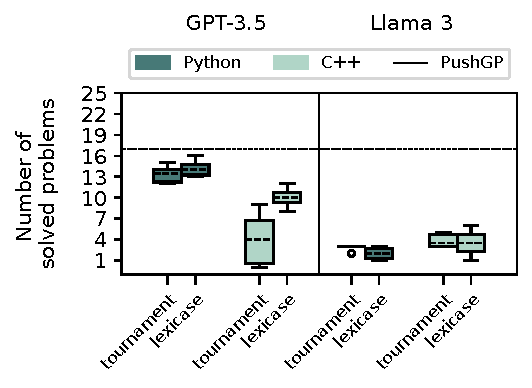
\includegraphics[width=\linewidth, trim={0mm 4mm 0mm 0mm}]{img/results/lexicase/num_solved_problem_lexicase_psb2_6runs_boxplot_v5.pdf}
  \caption{PSB2.}
    % \vspace{14pt}
  \label{fig:num-solved-lexicase-selection-psb2}
\end{subfigure}
% 
\begin{subfigure}{.45\linewidth}
\centering
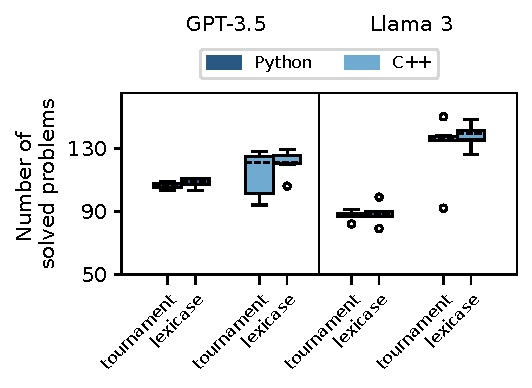
\includegraphics[width=\linewidth, trim={0mm 4mm 0mm 0mm}]{img/results/lexicase/num_solved_problem_lexicase_humaneval_6runs_boxplot_v5.pdf}
  \caption{HumanEval.}
    % \vspace{14pt}
  \label{fig:num-solved-lexicase-selection-he}
\end{subfigure}
\caption{Number of solved problems in lexicase and tournament selection experiments for \method{} with GPT-3.5 and Llama 3 and fixed tree-arity $N^*$.}
\label{fig:num-solved-lexicase-selection}
\end{figure}
\begin{figure}[bt]
% 
\begin{subfigure}{.45\linewidth}
\centering
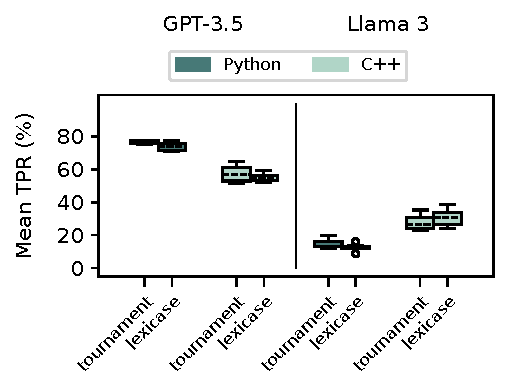
\includegraphics[width=\linewidth, trim={0mm 4mm 0mm 0mm}]{img/results/mean_tpr/mean_tpr_lexicase_psb2_6runs_boxplot_v5.pdf}
  \caption{PSB2.}
  \label{fig:mean-tpr-lexicase-selection-psb2}
\end{subfigure}
% 
\begin{subfigure}{.45\linewidth}
\centering
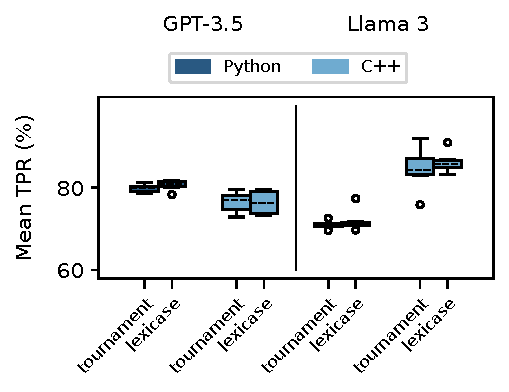
\includegraphics[width=\linewidth, trim={0mm 4mm 0mm 0mm}]{img/results/mean_tpr/mean_tpr_lexicase_humaneval_6runs_boxplot_v5.pdf}
  \caption{HumanEval.}
  \label{fig:mean-tpr-lexicase-selection-he}
\end{subfigure}
\caption{Mean $TPR$ (measured in \%) in lexicase and tournament selection experiments for \method{} with GPT-3.5 and Llama 3 and fixed tree-arity $N^*.$}
\label{fig:mean-tpr-lexicase-selection}
\end{figure}

\begin{figure}[t]
\centering
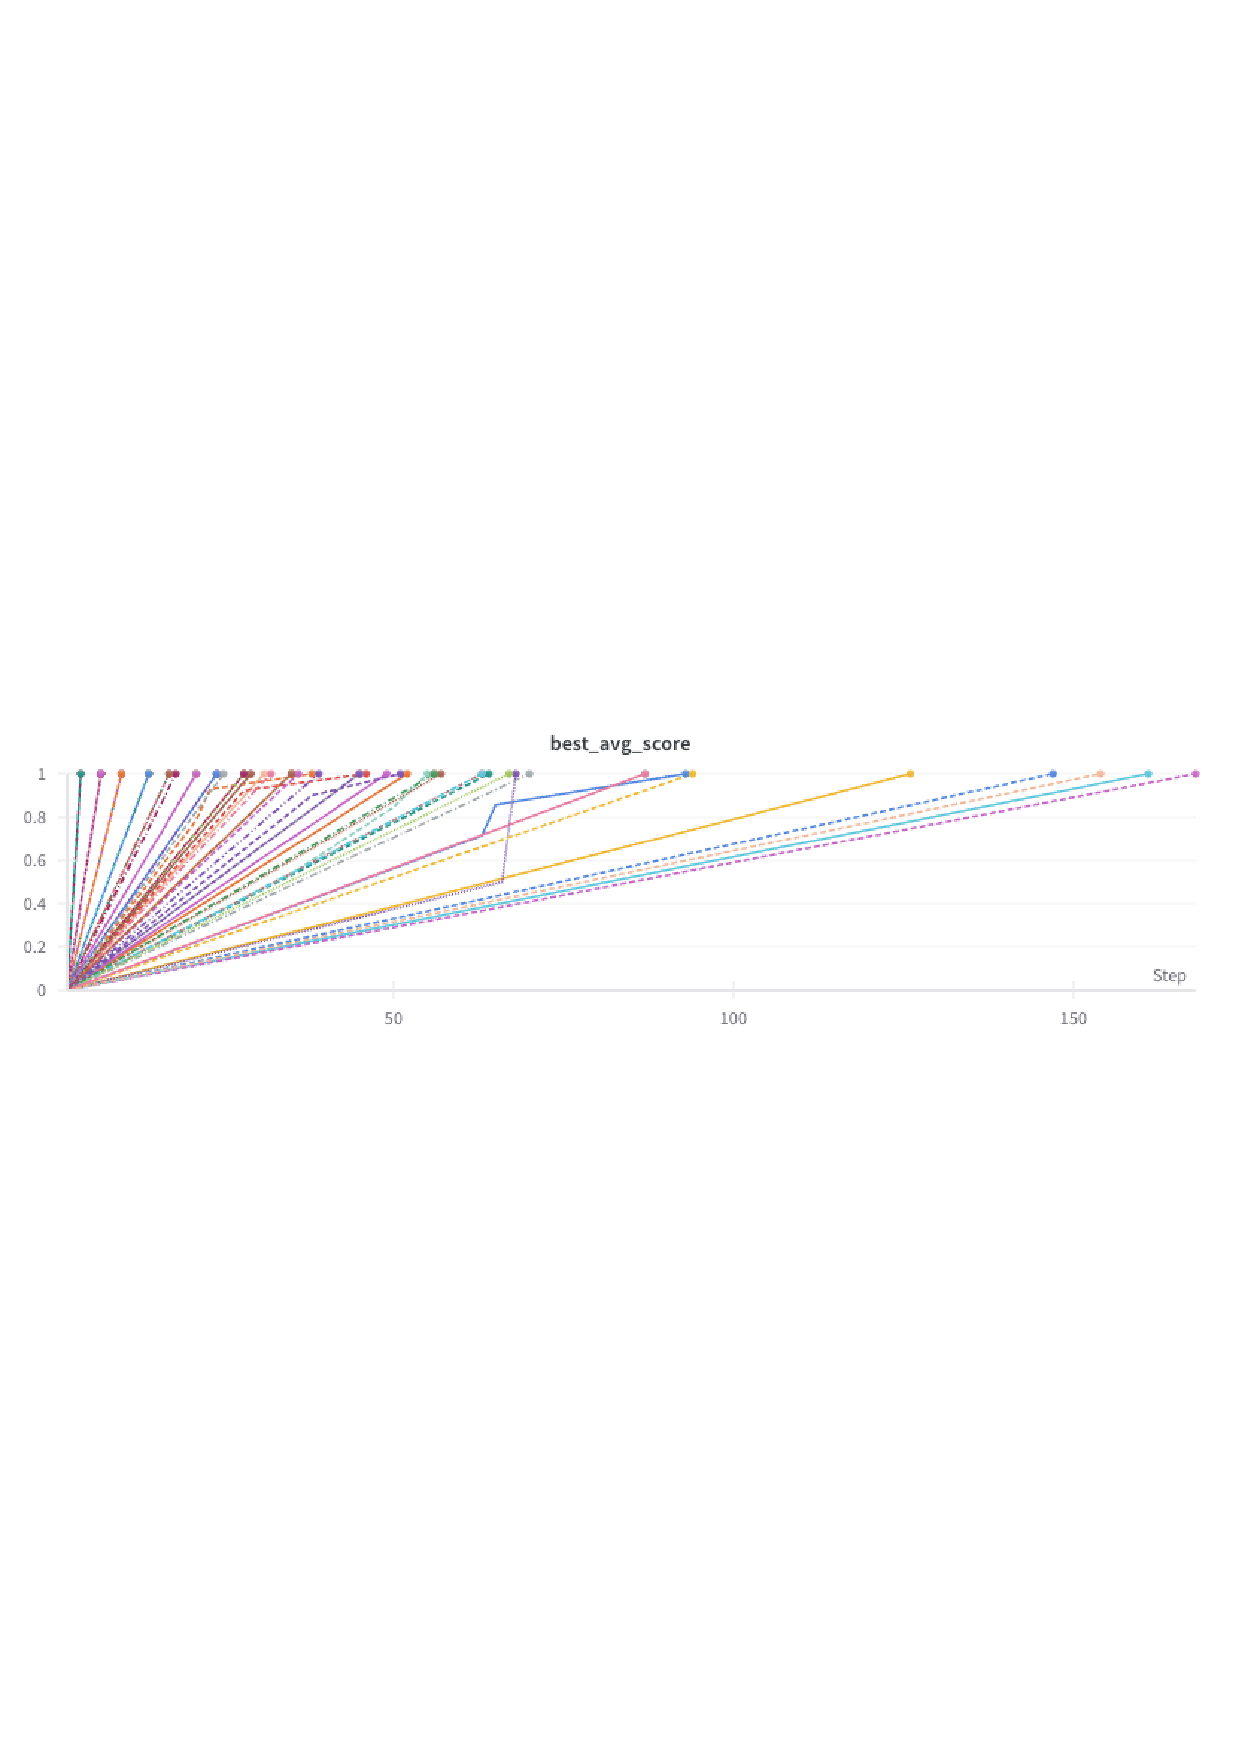
\includegraphics[width=\linewidth, trim={2mm 123mm 3mm 130mm}, clip]{img/results/best_avg_score_lexicase/best-avg-score-seidr-telo-humaneval-gpt-3.5-turbo-run3.pdf}
\caption{The best score on validation tests (y-axis) obtained up to an indicated logging step (x-axis) for problems solved from the second or later attempts with lexicase selection using \method{} with \gpt{}. Results are obtained for HumanEval. ``Step'' on the x-axis corresponds to logging settings and roughly indicates the speed of finding solutions to different problems. Each line stands for a unique solution.}
\label{fig:lexicase-tpr-jumps}
\end{figure}


\begin{framed}
\textbf{Parent selection strategies for \method{} with GPT-3.5 and \llama{} in the generalizability experiments (RQ3, RQ4, RQ5):} 
No leading ranking strategy is found for \method{} experiments with GPT-3.5 and \llama{} as measured by the average test pass rate and the average number of solved problems over six runs. 
In the vast majority of experiments where a solution is found and at least one debugging attempt is made, the score jumps from 0 to 1 as opposed to climbing up incrementally and makes ranking strategy less impactful than effective prompting. 
\end{framed}

\subsubsection{Overall Generalizability of \method{} with parent selection strategies and repair-replace trade-off.}
\label{sec:seidr-overall-generalizability}

We combine all the results together in Table~\ref{tab:generalizability-psb2} for PSB2 and Table~\ref{tab:generalizability-he} for HumanEval-X, where we show the number of solved problems at different cutoffs ($k$). 
An average is taken over all runs for the experiments with multiple restarts, and results for one run are shown for \method{} with Codex. 
We compare the performance of PSB2 solutions synthesized with \method{} to the PushGP genetic programming system with down-sampled lexicase selection~\cite{helmuth2022:problemsolving}. 
To compare performance of \method{} with other LLMs without \method{}, we report average percentage of solved problems for HumanEval-X. 
For HumanEval-X, we cite the performance of the state-of-the-art models as reported by their authors without \method{}, such as CodeGeex~\cite{zheng2023:codegeex}, GPT-3.5 and GPT-4~\cite{openai2023:gpt4}, for reference, and compare \method{} with GPT-3.5 and Code Llama~\cite{roziere2023:code} results at different cutoffs ($k$ for $pass@k$).
Additionally, we report the number of solved problems in the union of all experiments for a given dataset, model, and language, because different problems are solved in different restarts of the method. We refer to these results as ``solved at least once'' further in the text.

In PSB2-Python experiments, \method{} with Codex has larger pass@1000 than the maximum pass@100 measured for \method{} with \gpt{}. \method{} with Codex also solves 20 problems at least once, whereas \method{} with \gpt{} solves 18.
\method{} with Codex also outperforms other LLMs on PSB2 in C++.
No parent selection strategy or tree-arity $N^*$ is leading across all PSB2 experiments. 

In the HumanEval-C++ experiments, \method{} performs well at larger $k,$ i.e., when debugging steps are made. 
Remarkably, the union of \method{} experiments with both \gpt{} and a much smaller \llama{} solve 163 problems (or 99.4\% in Table~\ref{tab:generalizability-he}) and 162 problems (or 98.8\%) in HumanEval-C++, correspondingly.
\method{} does not outperform other LLMs on HumanEval-Python, which, as mentioned earlier, could be the effect of HumanEval-Python being a popular benchmark for testing LLMs and indirectly optimizing the models.

\begin{table}[b]
    \centering
    \caption{Average number of solved PSB2 problems using \method{} with different LLMs and PushGP. The best results among \method{}-only experiments at each $k$ are highlighted in bold. The best scores obtained in a single run are underlined. If pass@100 is not available, we cite the best available results in brackets. $N^*$ stands for the number of debug candidates and debug instructions to generate (tree-arity).}\small
    \label{tab:generalizability-psb2}
\begin{adjustbox}{max width=.92\textwidth}
\begin{DIFnomarkup} %% turn off latexdiff
\begin{tabular}{llllrrr}
\toprule
Language & Model in \method{} & $N^*$ & Parent selection &  pass@1 &  pass@10 &  pass@100 \\
\midrule
% 
Python & \gpt{} & 1   &         tournament &    10.5 &     12.0 &      12.0 \\
    &        & 2   &         tournament &     9.3 &     11.5 &      12.0 \\
    &        & 4   &         tournament &     9.8 &     12.2 &      13.3 \\
    &        & 10  &         tournament &    10.7 &     \textbf{12.7} &      \textbf{14.5} \\
    &        & 16  &         tournament &    10.0 &     11.3 &      13.3 \\
    &        & 16  &           lexicase &    10.2 &     12.3 &      14.2 \\
    &        & 100 &         tournament &    \textbf{10.8} &     12.2 &      13.7 \\
\cline{3-7}\\[-8pt]
    &  \multicolumn{3}{l}{solved at least once by \method{} with \gpt{}} &  13 &       17 &       18 \\[1pt]
\cline{2-7}\\[-8pt]
        & Codex  & 10 & tournament &      5 &       10 &        14 (pass@1000=\underline{19}) \\[1pt]
\cline{3-7}\\[-8pt]
       &  \multicolumn{3}{l}{solved at least once by \method{} with Codex}   & 8 &       13 &        17 (pass@1000=20) \\[3pt]
\cline{2-7}\\[-8pt]
        &  PushGP (no \method{})   &    -            &       - &        - &       - &  (17)\\[1pt]
\cline{2-7}\\[-8pt]
% 
        & \llama{} & 1   &         tournament &     1.2 &      1.3 &       2.3 \\
        &        & 2   &         tournament &     1.0 &      1.5 &       1.5 \\
        &        & 4   &         tournament &     1.0 &      1.5 &       2.3 \\
        &        & 10  &         tournament &     1.5 &      2.0 &       2.2 \\
        &        & 16  &         tournament &     \textbf{1.7} &      \textbf{2.8} &       2.8 \\
        &        & 16  &           lexicase &     1.0 &      1.7 &       2.0 \\
        &        & 100 &         tournament &     1.0 &      1.0 &       \textbf{3.8} \\[1pt]
\cline{3-7}\\[-8pt]
    &  \multicolumn{3}{l}{solved at least once by \method{} with \llama{}} &   4 &        5 &       11 \\
\midrule\\[-8pt]
 C++ & GPT-3.5 & 1   &         tournament &     0.0 &      5.6 &       5.5 \\
       &        & 2   &         tournament &     1.0 &      5.0 &       6.0 \\
       &        & 2   &           lexicase &     \textbf{1.3} &     \textbf{ 9.0} &      \textbf{10.0} \\
       &        & 4   &         tournament &     1.0 &      4.6 &       6.8 \\
       &        & 10  &         tournament &     1.0 &      1.3 &       5.6 \\
       &        & 16  &         tournament &     1.0 &      1.2 &       8.3 \\
       &        & 100 &         tournament &     1.0 &      1.2 &       2.3 \\[1pt]
\cline{3-7}\\[-8pt]
       & \multicolumn{3}{l}{solved at least once by \method{} with \gpt{}}   & 2 &       13 &       13 \\[1pt]
% 
\cline{2-7}\\[-8pt]
   & Codex  & 10 & tournament &     3 &       12 &   14 (pass@1000=\underline{17})\\[1pt]
\cline{3-7}\\[-8pt]
       & \multicolumn{3}{l}{solved at least once by \method{} with Codex}   & 10 &       12 &        15 (pass@1000=18) \\[1pt]
\cline{2-7}\\[-8pt]
   &  PushGP (no \method{}) & -   &    -            &       - &        - &      (\underline{17})\\[1pt]
\cline{2-7}\\[-8pt]
        & Llama 3 & 1   &         tournament &     0.0 &      1.0 &       2.0 \\
       &        & 2   &         tournament &     0.0 &      \textbf{2.0} &       2.8 \\
       &        & 4   &         tournament &     \textbf{1.0} &     \textbf{ 2.0} &       2.6 \\
       &        & 10  &         tournament &     \textbf{1.0} &      1.4 &       \textbf{4.0} \\
       &        & 16  &         tournament &     0.0 &      1.8 &       3.8 \\
       &        & 16  &           lexicase &    \textbf{ 1.0} &      1.4 &       3.5 \\
       &        & 100 &         tournament &     0.0 &      0.0 &       3.7 \\[1pt]
\cline{3-7}\\[-8pt]
       & \multicolumn{3}{l}{solved at least once by \method{} with \llama{}}  & 4 &        5 &       11  \\
\bottomrule
\end{tabular}
\end{DIFnomarkup} %% turn off latexdiff
\end{adjustbox}
\end{table}



% \begin{table}[t]
%     \centering
%     \caption{Number of solved tasks in HumanEval-X using \method{} with different LLMs. The best results among \method{}-only experiments at each $k$ are highlighted in bold.The best scores for each language are underlined. If pass@100 is not available, the best reported results are mentioned as in the corresponding papers. $N^*$ stands for the number of debug candidates and debug instructions to generate (tree-arity).}\small
%     \label{tab:generalizability-he}
% \begin{adjustbox}{max width=\textwidth}
% \begin{tabular}{llllrrr}
% \toprule
% Language & Model & $N^*$ & Ranking &  pass@1 &  pass@10 &  pass@100 \\
% \midrule
% Python & \gpt{} & 1   &         tournament &    87.5 &     \textbf{99.0} &     103.8 \\
%        &        & 2   &         tournament &    84.2 &     95.5 &     104.5 \\
%        &        & 4   &         tournament &    85.5 &     95.8 &     106.3 \\
%        &        & 4   &           lexicase &    86.2 &     97.7 &     \textbf{108.3} \\
%        &        & 10  &         tournament &    83.8 &     95.7 &     101.2 \\
%        &        & 16  &         tournament &    87.0 &     97.7 &     104.2 \\
%        &        & 100 &         tournament &    \textbf{88.5} &     93.0 &     102.5 \\[1pt]
% \cline{3-7}\\[-8pt]
%        &      & all $N^*$ & all strategies   & 116 &      138 &      144 \\[1pt]
% \cline{2-7}\\[-8pt]
%     &   Llama 3 & 1   &         tournament &    36.0 &     72.2 &      77.2 \\
%        &        & 2   &         tournament &    39.3 &     \textbf{79.5} &      85.0 \\
%        &        & 4   &         tournament &    36.8 &     70.7 &      85.0 \\
%        &        & 10  &         tournament &    39.3 &     70.3 &      87.3 \\
%        &        & 10  &           lexicase &    \textbf{43.0} &     72.3 &      \textbf{88.7} \\
%        &        & 16  &         tournament &    38.5 &     68.2 &      84.5 \\
%        &        & 100 &         tournament &    35.2 &     43.2 &      78.7  \\[1pt]
% \cline{3-7}\\[-8pt]
%        &      & all $N^*$ & all strategies   & 93 &      121 &      130 \\[1pt]
% \midrule\\[-8pt]
% C++    & \gpt{} & 1   &         tournament &     5.5 & \textbf{91.7} &  \textbf{128.7} \\
%        &        & 2   &         tournament &  \textbf{7.7} &     60.0 &     114.2 \\
%        &        & 2   &           lexicase &     7.0 &     58.8 &     120.7 \\
%        &        & 4   &         tournament &     7.3 &     45.5 &     103.2 \\
%        &        & 10  &         tournament &     5.8 &     22.5 &      81.5 \\
%        &        & 16  &         tournament &     7.3 &     21.7 &      83.8 \\
%        &        & 100 &         tournament &     5.8 &     11.7 &      51.3 \\[1pt]
% \cline{3-7}\\[-8pt]
%        &      & all $N^*$ & all strategies   & 33 &      146 &      163 \\[1pt]
% \cline{2-7}\\[-8pt]
%     &   Llama 3 & 1   &         tournament &    \textbf{48.5} &     \textbf{97.5} &     130.3 \\
%        &        & 2   &         tournament &    30.5 &     84.7 &     117.2 \\
%        &        & 4   &         tournament &    32.8 &     83.0 &     121.2 \\
%        &        & 10  &         tournament &    42.0 &     92.5 &     131.2 \\
%        &        & 10  &           lexicase &    42.5 &     99.8 &     \textbf{138.2} \\
%        &        & 16  &         tournament &    34.3 &     87.0 &     123.8 \\
%        &        & 100 &         tournament &    44.5 &     65.2 &     129.8 \\[1pt]
% \cline{3-7}\\[-8pt]
%        &      & all $N^*$ & all strategies   & 118 &      160 &      162 \\[1pt]
% \bottomrule
% \vspace{-3.4ex}
% \end{tabular}
% \end{adjustbox}
% \end{table}





\begin{table}[t]
    \centering
    \caption{Percentage of solved tasks in HumanEval-X using \method{} with different LLMs. The best results among \method{}-only experiments at each $k$ are highlighted in bold. The best scores obtained in a single run are underlined. $N^*$ stands for the number of debug candidates and debug instructions to generate (tree-arity).}\small
    \label{tab:generalizability-he}
    \vspace{-1.4ex}
\begin{adjustbox}{max width=\textwidth}
\begin{DIFnomarkup} %% turn off latexdiff
\begin{tabular}{llllrrr}
\toprule
Language & Model in \method{} & $N^*$ & Ranking &  pass@1 &  pass@10 &  pass@100 \\
\midrule
Python & \gpt{} & 1   &         tournament &    53.4 &     \textbf{60.4} &      63.3 \\
       &        & 2   &         tournament &    51.3 &     58.2 &      63.7 \\
       &        & 4   &         tournament &    52.1 &     58.4 &      64.8 \\
       &        & 4   &           lexicase &    52.5 &     59.6 &      \textbf{66.1} \\
       &        & 10  &         tournament &    51.1 &     58.3 &      61.7 \\
       &        & 16  &         tournament &    53.0 &     59.6 &      63.5 \\
       &        & 100 &         tournament &    \textbf{54.0} &     56.7 &      62.5 \\[1pt]
\cline{3-7}\\[-8pt]
       & \multicolumn{3}{l}{solved at least once by \method{} with \gpt{}}   & 70.7 &     84.1 &      87.8 \\[1pt]
\cline{2-7}\\[-8pt]
    &   Llama 3 & 1   &         tournament &    22.0 &     44.0 &      47.1 \\
       &        & 2   &         tournament &    24.0 &     \textbf{48.5 }&      51.8 \\
       &        & 4   &         tournament &    22.5 &     43.1 &      51.8 \\
       &        & 10  &         tournament &    24.0 &     42.9 &      53.3 \\
       &        & 10  &           lexicase &    \textbf{26.2} &     44.1 &      \textbf{54.1} \\
       &        & 16  &         tournament &    23.5 &     41.6 &      51.5 \\
       &        & 100 &         tournament &    21.4 &     26.3 &      48.0  \\[1pt]
\cline{3-7}\\[-8pt]
       & \multicolumn{3}{l}{solved at least once by \method{} with \llama{}} & 56.7 &     73.8 &      79.3 \\[1pt]
\cline{2-7}\\[-8pt]
& \multicolumn{6}{l}{\textbf{LLM results without \method{}}} \\
 & GPT-3.5 (ChatGPT) & - &  - &  48.1  &  -   &    - \\
 & GPT-4 & - &  - & \underline{67.0}   &  -   &    - \\
 & Code Llama 34B & - &  - &  48.8  &  76.8   &    93.0 \\
 & Unnatural Code Llama 34B & - &  - &  62.2  &  \underline{85.2}   &    \underline{95.4} \\
 & CodeGeeX & - &  - &  22.89  &  39.57   &    60.92 \\[-2pt]
\midrule\\[-12pt]
C++    & \gpt{} & 1   &         tournament &     3.4 &    \textbf{ 55.9} &      \textbf{78.5} \\
       &        & 2   &         tournament &     \textbf{4.7} &     36.6 &      69.6 \\
       &        & 2   &           lexicase &     4.3 &     35.9 &      73.6 \\
       &        & 4   &         tournament &     4.5 &     27.7 &      62.9 \\
       &        & 10  &         tournament &     3.6 &     13.7 &      49.7 \\
       &        & 16  &         tournament &     4.5 &     13.2 &      51.1 \\
       &        & 100 &         tournament &     3.6 &      7.1 &      31.3 \\[1pt]
\cline{3-7}\\[-8pt]
       & \multicolumn{3}{l}{solved at least once by \method{} with \gpt{}} & 20.1 &     89.0 &      99.4 \\[1pt]
\cline{2-7}\\[-8pt]
    &   Llama 3 & 1   &         tournament &    \textbf{29.6} &     59.5 &      79.5 \\
       &        & 2   &         tournament &    18.6 &     51.6 &      71.4 \\
       &        & 4   &         tournament &    20.0 &     50.6 &      73.9 \\
       &        & 10  &         tournament &    25.6 &     56.4 &      80.0 \\
       &        & 10  &           lexicase &    25.9 &     \underline{\textbf{60.9}} &      \underline{\textbf{84.2}} \\
       &        & 16  &         tournament &    20.9 &     53.0 &      75.5 \\
       &        & 100 &         tournament &    27.1 &     39.7 &      79.2 \\[1pt]
\cline{3-7}\\[-8pt]
       & \multicolumn{3}{l}{solved at least once by \method{} with \llama{}} & 72.0 &     97.6 &      98.8  \\[1pt]
\cline{2-7}\\[-8pt]
& \multicolumn{6}{l}{\textbf{LLM results without \method{}}} \\
& Code Llama 34B & - &  - &  \underline{47.8}  &  -   &    - \\
& CodeGeeX & - &  - &  17.06  &  32.21   &    51.00 \\[-2pt]
\bottomrule
\vspace{-4.4ex}
\end{tabular}
\end{DIFnomarkup} %% turn off latexdiff
\end{adjustbox}
\end{table}

\begin{framed}
\textbf{Summary of \method{} results:} 
\method{} with Codex benefits from the repair-replace trade-off when building a search tree of PSB2 solutions. The best results on PSB2 are achieved with Codex, tree-arity of 10 and a maximum of 1000 programs generated. A trend of having the best tree-arity set to 10 does not fully hold for other tested models, \gpt{} and \llama{}, where different tree arities performed better in different settings, e.g., depending on the parent selection algorithm, dataset, and programming language. 
Due to increasing costs of newer models time required for testing, we have run \gpt{} and \llama{} 6 times with each set of hyperparameters and stopped building the search tree at 100 programs. 
In HumanEval-C++, the union of these runs has solved 163 problems with \gpt{}, 162 problems with a much smaller \llama{}-8B model.
\method{} runs has also solved 18 PSB2 problems in C++ and 20 in Python with Codex at least once over all the experiments. 
The numbers for \method{} with \gpt{} are lower than for Codex, possibly due to a focus of \gpt{} on general reasoning and of Codex --- on coding.
A smaller \llama{} model performs poorly on PSB2, which we appoint to the difficulty of the benchmark and the fact that HumanEval is a popular dataset to compare the models on, so the models can be indirectly optimized for higher performance on HumanEval than on other programming benchmarks.
\end{framed}


\subsection{Threats to Validity}
\label{sec:seidr-threats}

External threats to validity concern \method{} performance on different other benchmarks and the use of more language models than the tested ones. 
Specifically, PSB2 and HumanEval-X contain programming tasks which require smaller functions to be generated than production-scale software.
While some canonical solutions provided in HumanEval-Python have been criticised~\cite{liu2023:your}, we primarily use unit tests to evaluate the output of \method{}. Therefore, their weaknesses do not impact our results.
% We plan to extend our experiments in future work to explore the generalizability of results to more complex benchmarks.

Internal threats relate to the implementation.
We use PSB2, which has both corner cases and regular tests available. 
To ensure a fair comparison with other studies on PSB2, we evaluate and report results on the provided test set of PSB2, of which we randomly pick 2000 tests. 
A risk that a program does not pass other tests than the picked once persists but is assumed low given the large enough number of 2000 tests. 

The large language models for code editing and text completion used in this study are non-deterministic, 
which can affect the results. 
Due to prohibitive model inference costs and discontinuation of support for earlier models, each experiment with Codex and GPT-3 is run only once. 
Experiments with \llama{} and \gpt{} are restarted six times. 
We acknowledge that more restarts can yield a more thorough picture of the models' performance, although it is not the standard practice in the LLM domain~\cite{ouyang2023:llm}.
Our temperature-based sampling procedure described in Section\ref{sec:seidr-synth} reduces this stochasticity significantly, especially for low-EPG results, because earlier solutions in the search tree are obtained with lower temperatures, and lower temperature limits the stochasticity.
Codex, GPT-3, and GPT-3.5 are black-box models and can generate malicious code~\cite{pearce2022:asleep}. 
Therefore, when coding in real life, the models' output should be carefully reviewed before running it.
% \ag{The Codex model was pre-trained on an unbalanced dataset across programming languages~\cite{chen2021:evaluating}. Thus, 

The results can be skewed towards high performance in the programming languages prevailing in the pre-training dataset used by authors of the tested LLMs --- an issue also known as \emph{data contamination}.
However, if the models were to directly reproduce all the seen solutions from the training data as they are, the seen problems would have been solved from the first attempt.
Since we observe $EPG>1$ values, data contamination is likely to have only a partial effect on the results.
Moreover, the results can be affected by popular evaluation benchmarks: even though the benchmarks themselves are usually not parts of the pre-training dataset, the published LLMs are likely to be optimized for high performance on these benchmarks.   

\section{Conclusion}
\label{sec:seidr-conclusion}

In this study, we propose \method{}, the multi-agent framework to solve the challenge of fully autonomous programming. 
In SEIDR, the program synthesis procedure is augmented from the direct generation of code with large language models instructions to iterative calls to a \debug{} agent with a successive \rank{} component. 
The \debug{} agent performs a tree search across program candidates generated by a large language model for code.
The LLM used for code repair takes imperfect program candidates and instructions for their improvement as prompts. 
The instructions are obtained from both static templates with failing test case descriptions and templates with auto-generated bug summaries by a text completion language model. 
We explore 11 prompting strategies and the repair-replace trade-off of updating the draft program.

In addition to the initial exploration of hyperparameters that influence population size at each generation and number of children for each parent in \method{} iterations, we extend the framework to test a total of two different ranking strategies (tournament selection and lexicase selection), three models in the coding part of \method{} (Codex, \gpt{} and \llama{}), two datasets (PSB2 and HumanEval-X), two programming languages (Python and C++), and various branching factors. 
With the update to the newer models, prompting strategies and parameters of the tree search are updated accordingly. 

\head{Contributions}
We run one set of initial exploration experiments and two sets of generalizability experiments. 
In the initial exploration, we test \method{} with the Codex-edit as the model for draft program synthesis and debugging in Python and C++ on the PSB2 benchmark. 
In our experiments, \method{} outperforms the PushGP baseline and achieves the state-of-the-art result with 19 solved problems out of 25. 
It requires under 1000 program executions to solve them, in stark contrast to billions\footnote{~A problem is considered "solved" by PushGP if at least 1 of 100 runs, each with a limit of 60 million programs, was successful.} of executions in PushGP, making it feasible in the areas with costly testing, such as robotics.
Investigation of the repair-replace trade-off shows that \method{} with tree-arity of 10 outperforms both the replace-only strategy and the repair-only approach. 
Our prompt engineering study shows that bug summaries generated with ``confidence indicators,'' such as ``obviously'' improve the performance of \method{} during C++ code synthesis. 
% Overall, our framework shows low performance variability with different prompts, which indicates its robustness.%

To study generalizability of \method{}, we use experiment with GPT-3.5 and Llama 3-8B as the models for draft program synthesis, explaining errors in synthesized programs and their debugging in Python and C++ on the PSB2 and HumanEval-X benchmarks. 
Our experiments with lexicase and tournament parent selection in the \rank{} agent do not show consistent improvement with either of the parent selection policies or tree-arity values. 
One observation is that program candidates in generations prior to the final solution do not pass any test in the test suite in the vast majority of cases. 
The test pass rate for the final solution abruptly increases in one generation from 0 to all tests passed. 

In our generalizability experiments, \method{} does not outperform the state-of-the-art baselines for PSB2 and HumanEval-Python but shows better performance than using LLMs without \method{} with the same prompts as in \method{}.
The method achieves high results of 78.5\% average pass@100 on HumanEval-C++ with \gpt{} and 84.2\% with \llama{}.
Remarkably, in HumanEval-C++, the union of \method{} restarts with different hyperparameters has solved 163 problems with \gpt{}, 162 problems with a much smaller \llama{}-8B model.
The union of \method{} runs has solved 18 PSB2 problems in C++ and 20 in Python with Codex. 
% Moreover, the method achieves the state-of-the-art result for pass@10 (74.44\%) with Code Llama 34B and for pass@100 (93.29\%) with GPT-3.5 on HumanEval-C++. 
% The approach requires under 100 program executions to obtain the reported results with GPT-3.5 and Code Llama.
% \method{} with moderate number of generated programs for each bug explanation is favorable both for obtaining a solution and for the speed of solving a task. 

\head{Future work}
Further investigation of \method{} generalizability and ranking strategies are some of the areas for future work. 
Benchmarks with more tests than in HumanEval-X may shed more light on the most effective choice of the number of programs generated from each bug explanation, as well as the framework's comparison on large-context projects. 
As an agent-based framework, \method{} shows how LLM-based agents and other non-LLM agents or components can collaboratively interact and solve software engineering tasks.

\section*{Data Availability}
To support open science and allow for replication and verification of our work, a replication package containing the code and results will be made publicly available in Zenodo.\footnote{~While the manuscript is under review, the replication package is made available as a shared Google Drive to allow for improvements \url{https://drive.google.com/drive/folders/1SP0CVJQ6CdktFtksVs7tYu9jdLHIjHxa?usp=sharing}. We have reserved Zenodo DOI \href{https://doi.org/10.5281/zenodo.13754705}{10.5281/zenodo.13754705} to upload it after the review process has concluded.
}
